%%%%%%%%%%%%%%%%%%%%%%%%%%%%%%%%%%%%%%%%
% datoteka diploma-vzorec.tex
%
% vzorčna datoteka za pisanje diplomskega dela v formatu LaTeX
% na UL Fakulteti za računalništvo in informatiko
%
% vkup spravil Gašper Fijavž, december 2010
% 
%
%
% verzija 12. februar 2014 (besedilo teme, seznam kratic, popravki Gašper Fijavž)
% verzija 10. marec 2014 (redakcijski popravki Zoran Bosnić)
% verzija 11. marec 2014 (redakcijski popravki Gašper Fijavž)
% verzija 15. april 2014 (pdf/a 1b compliance, not really - just claiming, Damjan Cvetan, Gašper Fijavž)
% verzija 23. april 2014 (privzeto cc licenca)
% verzija 16. september 2014 (odmiki strain od roba)
% verzija 28. oktober 2014 (odstranil vpisno številko)
% verija 5. februar 2015 (Literatura v kazalu, online literatura)
% verzija 25. september 2015 (angl. naslov v izjavi o avtorstvu)
% verzija 26. februar 2016 (UL izjava o avtorstvu)
% verzija 16. april 2016 (odstranjena izjava o avtorstvu)
% verzija 5. junij 2016 (Franc Solina dodal vrstice, ki jih je označil s svojim imenom)


\documentclass[a4paper, 12pt]{book}

\usepackage[utf8x]{inputenc}   % omogoča uporabo slovenskih črk kodiranih v formatu UTF-8
\usepackage[slovene,english]{babel}    % naloži, med drugim, slovenske delilne vzorce
\usepackage[pdftex]{graphicx}  % omogoča vlaganje slik različnih formatov
\usepackage{fancyhdr}          % poskrbi, na primer, za glave strani
\usepackage{amssymb}           % dodatni simboli
\usepackage{amsmath}           % eqref, npr.
%\usepackage{hyperxmp}
\usepackage[hyphens]{url}  % dodal Solina
\usepackage{comment}       % dodal Solina
\usepackage{fancyvrb}

\usepackage[pdftex, colorlinks=true,
						citecolor=black, filecolor=black, 
						linkcolor=black, urlcolor=black,
						pagebackref=false, 
						pdfproducer={LaTeX}, pdfcreator={LaTeX}, hidelinks]{hyperref}

\usepackage{color}       % dodal Solina
\usepackage{soul}       % dodal Solina

%%%%%%%%%%%%%%%%%%%%%%%%%%%%%%%%%%%%%%%%
%	DIPLOMA INFO
%%%%%%%%%%%%%%%%%%%%%%%%%%%%%%%%%%%%%%%%
\newcommand{\ttitle}{Optimizacija strojne kode brez časovnih omejitev}
\newcommand{\ttitleEn}{Optimization of the machine code without time constraint}
\newcommand{\tsubject}{\ttitle}
\newcommand{\tsubjectEn}{\ttitleEn}
\newcommand{\tauthor}{Franko Jančič}
\newcommand{\tkeywords}{računalnik, superoptimizator, strojna koda,prevajalnik,optimizacija}
\newcommand{\tkeywordsEn}{computer,superoptimizator,machine code,asembler,optimization}


%%%%%%%%%%%%%%%%%%%%%%%%%%%%%%%%%%%%%%%%
%	HYPERREF SETUP
%%%%%%%%%%%%%%%%%%%%%%%%%%%%%%%%%%%%%%%%
\hypersetup{pdftitle={\ttitle}}
\hypersetup{pdfsubject=\ttitleEn}
\hypersetup{pdfauthor={\tauthor, matjaz.kralj@fri.uni-lj.si}}
\hypersetup{pdfkeywords=\tkeywordsEn}


 


%%%%%%%%%%%%%%%%%%%%%%%%%%%%%%%%%%%%%%%%
% postavitev strani
%%%%%%%%%%%%%%%%%%%%%%%%%%%%%%%%%%%%%%%%  

\addtolength{\marginparwidth}{-20pt} % robovi za tisk
\addtolength{\oddsidemargin}{40pt}
\addtolength{\evensidemargin}{-40pt}

\renewcommand{\baselinestretch}{1.3} % ustrezen razmik med vrsticami
\setlength{\headheight}{15pt}        % potreben prostor na vrhu
\renewcommand{\chaptermark}[1]%
{\markboth{\MakeUppercase{\thechapter.\ #1}}{}} \renewcommand{\sectionmark}[1]%
{\markright{\MakeUppercase{\thesection.\ #1}}} \renewcommand{\headrulewidth}{0.5pt} \renewcommand{\footrulewidth}{0pt}
\fancyhf{}
\fancyhead[LE,RO]{\sl \thepage} 
%\fancyhead[LO]{\sl \rightmark} \fancyhead[RE]{\sl \leftmark}
\fancyhead[RE]{\sc \tauthor}              % dodal Solina
\fancyhead[LO]{\sc Diplomska naloga}     % dodal Solina


\newcommand{\BibTeX}{{\sc Bib}\TeX}

%%%%%%%%%%%%%%%%%%%%%%%%%%%%%%%%%%%%%%%%
% naslovi
%%%%%%%%%%%%%%%%%%%%%%%%%%%%%%%%%%%%%%%%  


\newcommand{\autfont}{\Large}
\newcommand{\titfont}{\LARGE\bf}
\newcommand{\clearemptydoublepage}{\newpage{\pagestyle{empty}\cleardoublepage}}
\setcounter{tocdepth}{1}	      % globina kazala

%%%%%%%%%%%%%%%%%%%%%%%%%%%%%%%%%%%%%%%%
% konstrukti
%%%%%%%%%%%%%%%%%%%%%%%%%%%%%%%%%%%%%%%%  
\newtheorem{izrek}{Izrek}[chapter]
\newtheorem{trditev}{Trditev}[izrek]
\newenvironment{dokaz}{\emph{Dokaz.}\ }{\hspace{\fill}{$\Box$}}

%%%%%%%%%%%%%%%%%%%%%%%%%%%%%%%%%%%%%%%%%%%%%%%%%%%%%%%%%%%%%%%%%%%%%%%%%%%%%%%
%% PDF-A
%%%%%%%%%%%%%%%%%%%%%%%%%%%%%%%%%%%%%%%%%%%%%%%%%%%%%%%%%%%%%%%%%%%%%%%%%%%%%%%

%%%%%%%%%%%%%%%%%%%%%%%%%%%%%%%%%%%%%%%% 
% define medatata
%%%%%%%%%%%%%%%%%%%%%%%%%%%%%%%%%%%%%%%% 
\def\Title{\ttitle}
\def\Author{\tauthor, matjaz.kralj@fri.uni-lj.si}
\def\Subject{\ttitleEn}
\def\Keywords{\tkeywordsEn}

%%%%%%%%%%%%%%%%%%%%%%%%%%%%%%%%%%%%%%%% 
% \convertDate converts D:20080419103507+02'00' to 2008-04-19T10:35:07+02:00
%%%%%%%%%%%%%%%%%%%%%%%%%%%%%%%%%%%%%%%% 
\def\convertDate{%
    \getYear
}

{\catcode`\D=12
 \gdef\getYear D:#1#2#3#4{\edef\xYear{#1#2#3#4}\getMonth}
}
\def\getMonth#1#2{\edef\xMonth{#1#2}\getDay}
\def\getDay#1#2{\edef\xDay{#1#2}\getHour}
\def\getHour#1#2{\edef\xHour{#1#2}\getMin}
\def\getMin#1#2{\edef\xMin{#1#2}\getSec}
\def\getSec#1#2{\edef\xSec{#1#2}\getTZh}
\def\getTZh +#1#2{\edef\xTZh{#1#2}\getTZm}
\def\getTZm '#1#2'{%
    \edef\xTZm{#1#2}%
    \edef\convDate{\xYear-\xMonth-\xDay T\xHour:\xMin:\xSec+\xTZh:\xTZm}%
}

\expandafter\convertDate\pdfcreationdate 

%%%%%%%%%%%%%%%%%%%%%%%%%%%%%%%%%%%%%%%%
% get pdftex version string
%%%%%%%%%%%%%%%%%%%%%%%%%%%%%%%%%%%%%%%% 
\newcount\countA
\countA=\pdftexversion
\advance \countA by -100
\def\pdftexVersionStr{pdfTeX-1.\the\countA.\pdftexrevision}


%%%%%%%%%%%%%%%%%%%%%%%%%%%%%%%%%%%%%%%%
% XMP data
%%%%%%%%%%%%%%%%%%%%%%%%%%%%%%%%%%%%%%%%  
\usepackage{xmpincl}
\includexmp{pdfa-1b}

%%%%%%%%%%%%%%%%%%%%%%%%%%%%%%%%%%%%%%%%
% pdfInfo
%%%%%%%%%%%%%%%%%%%%%%%%%%%%%%%%%%%%%%%%  
\pdfinfo{%
    /Title    (\ttitle)
    /Author   (\tauthor, damjan@cvetan.si)
    /Subject  (\ttitleEn)
    /Keywords (\tkeywordsEn)
    /ModDate  (\pdfcreationdate)
    /Trapped  /False
}


%%%%%%%%%%%%%%%%%%%%%%%%%%%%%%%%%%%%%%%%%%%%%%%%%%%%%%%%%%%%%%%%%%%%%%%%%%%%%%%
%%%%%%%%%%%%%%%%%%%%%%%%%%%%%%%%%%%%%%%%%%%%%%%%%%%%%%%%%%%%%%%%%%%%%%%%%%%%%%%

\begin{document}
\selectlanguage{slovene}
\frontmatter
\setcounter{page}{1} %
\renewcommand{\thepage}{}       % preprecimo težave s številkami strani v kazalu
\newcommand{\sn}[1]{"`#1"'}                    % dodal Solina (slovenski narekovaji)

%%%%%%%%%%%%%%%%%%%%%%%%%%%%%%%%%%%%%%%%
%naslovnica
 \thispagestyle{empty}%
   \begin{center}
    {\large\sc Univerza v Ljubljani\\%
      Fakulteta za računalništvo in informatiko}%
    \vskip 10em%
    {\autfont \tauthor\par}%
    {\titfont \ttitle \par}%
    {\vskip 3em \textsc{DIPLOMSKO DELO\\[5mm]         % dodal Solina za ostale študijske programe
%    VISOKOŠOLSKI STROKOVNI ŠTUDIJSKI PROGRAM\\ PRVE STOPNJE\\ RAČUNALNIŠTVO IN INFORMATIKA}\par}%
    UNIVERZITETNI  ŠTUDIJSKI PROGRAM\\ PRVE STOPNJE\\ RAČUNALNIŠTVO IN INFORMATIKA}\par}%
%    INTERDISCIPLINARNI UNIVERZITETNI\\ ŠTUDIJSKI PROGRAM PRVE STOPNJE\\ RAČUNALNIŠTVO IN MATEMATIKA}\par}%
%    INTERDISCIPLINARNI UNIVERZITETNI\\ ŠTUDIJSKI PROGRAM PRVE STOPNJE\\ UPRAVNA INFORMATIKA}\par}%
%    INTERDISCIPLINARNI UNIVERZITETNI\\ ŠTUDIJSKI PROGRAM PRVE STOPNJE\\ MULTIMEDIJA}\par}%
    \vfill\null%
    {\large \textsc{Mentor}: doc.\ dr.  Peter Klepec\par}%
   {\large \textsc{Somentor}:  izr.\ prof.\ dr. Martin Krpan \par}%
    {\vskip 2em \large Ljubljana, 2016 \par}%
\end{center}
% prazna stran
%\clearemptydoublepage      % dodal Solina (izjava o licencah itd. se izpiše na hrbtni strani naslovnice)

%%%%%%%%%%%%%%%%%%%%%%%%%%%%%%%%%%%%%%%%
%copyright stran
\thispagestyle{empty}
\vspace*{8cm}
Fakulteta za računalništvo in informatiko podpira javno dostopnost znanstvenih, strokovnih in razvojnih rezultatov. Zato priporoča objavo dela pod katero od licenc, ki omogočajo prosto razširjanje diplomskega dela in/ali možnost nadaljne proste uporabe dela. Ena izmed možnosti je izdaja diplomskega dela pod katero od Creative Commons licenc \href{http://creativecommons.si}{http://creativecommons.si}

Morebitno pripadajočo programsko kodo praviloma objavite pod, denimo, licenco 
\emph{GNU General Public License, različica 3}. Podrobnosti licence so dostopne na spletni strani \href{http://www.gnu.org/licenses/}{http://www.gnu.org/licenses/}.

\begin{center}
\mbox{}\vfill
\emph{Besedilo je oblikovano z urejevalnikom besedil \LaTeX.}
\end{center}
% prazna stran
\clearemptydoublepage

%%%%%%%%%%%%%%%%%%%%%%%%%%%%%%%%%%%%%%%%
% stran 3 med uvodnimi listi
\thispagestyle{empty}
\vspace*{4cm}

\noindent
Fakulteta za računalništvo in informatiko izdaja naslednjo nalogo:
\medskip
\begin{tabbing}
\hspace{32mm}\= \hspace{6cm} \= \kill




Tematika naloge:
\end{tabbing}
Zaradi želje po hitrem prevajanju je optimizacija strojne kode med prevajanjem vedno časovno zelo omejena. Raziščite, ali bi z odpravo časovne omejitve pri optimizaciji strojne kode lahko pridobili bistveno učinkovitejšo strojno kodo glede na različne kriterije kot sta dolžina in hitrost kode. Preglejte ustrezno strokovno literaturo, podajte pregled in poskusite implementirati najobetavnejšo metodo, po možnosti tako, ki se jo da ustrezno paralelizirati.
\vspace{15mm}






\vspace{2cm}

% prazna stran
\clearemptydoublepage

%%%%%%%%%%%%%%%%%%%%%%%%%%%%%%%%%%%%%%%%
% kazalo
\pagestyle{empty}
\def\thepage{}% preprecimo tezave s stevilkami strani v kazalu
\tableofcontents{}


% prazna stran
\clearemptydoublepage

%%%%%%%%%%%%%%%%%%%%%%%%%%%%%%%%%%%%%%%%
% seznam kratic

\chapter*{Seznam uporabljenih kratic}  % spremenil Solina, da predolge vrstice ne gredo preko desnega roba

\begin{comment}
\begin{tabular}{l|l|l}
{\bf kratica} & {\bf angleško} & {\bf slovensko} \\ \hline
% after \\: \hline or \cline{col1-col2} \cline{col3-col4} ...
{\bf CA} & classification accuracy & klasifikacijska točnost \\
{\bf DBMS} & database management system & sistem za upravljanje podatkovnih baz \\
{\bf SVM} & support vector machine & metoda podpornih vektorjev \\
\dots & \dots & \dots \\
\end{tabular}
\end{comment}

\noindent\begin{tabular}{p{0.1\textwidth}|p{.4\textwidth}|p{.4\textwidth}}    % po potrebi razširi prvo kolono tabele na račun drugih dveh!
	{\bf kratica} & {\bf angleško} & {\bf slovensko} \\ \hline
	{\bf GCC}      & GNU Compiler Collection & GNU prevajalnikova knjižnjica \\
	{\bf GNU} & GNU's Not Unix & GNU-jev ne Unix \\
	{\bf CPU} & Computer Processing Unit & Centralno processna enota \\
	{\bf SA} & Simulated Annealing & Simulated Annealing \\
	{\bf DDEC} & Data-Driven Equivalence Checking & Podatkovno vodeno preverjanje ekvivalence  \\
	{\bf JIT} & Just-in-time & ravno pravi čas \\
	{\bf ULP} & uncertainty in the last place & odstopanja v zadnjem mestu \\
	{\bf GSO} & Group search optimizer  & skupinsko optimizaroe iskanja \\
	{\bf EGCS} & Experimental GNU Compiler System  & Eksperimentalni GNU prevajalni sistem \\
\end{tabular}
%%%%%%%%%%%%%%%%%%%%%%%%%%%%%%%%%%%%%%%%
% povzetek
\addcontentsline{toc}{chapter}{Povzetek}
\chapter*{Povzetek}

\noindent\textbf{Naslov:} \ttitle
\bigskip

\noindent\textbf{Avtor:} \tauthor
\bigskip

%\noindent\textbf{Povzetek:} 
\noindent 
V današnjem času nam je pisanje programov precej olajšano. Za pisanje lahko uporabimo visoko nivojske jezike (kot so Java, C, C++, Python itd) ali pa psevdo ukaze. Vendar moramo programe v večini primerov prevesti v strojno kodo, da jo lahko računalnik požene. Če pa bi si podrobno ogledali to strojno kodo, bi v nekaterih primerih opazili, da se prevedena koda ne ujema s izvorno kodo, klub temu, da je funkcijonalnost takega programa enaka kot v izvirni kodi. To je zato, ker ga prevajalnik optimizira. V nadaljevanju bomo spoznali koliko je možno program optimizirat v daljši časovni omejitvi in koliko se splača to delat.
\bigskip

\noindent\textbf{Ključne besede:} \tkeywords.
% prazna stran
\clearemptydoublepage

%%%%%%%%%%%%%%%%%%%%%%%%%%%%%%%%%%%%%%%%
% abstract
\selectlanguage{english}
\addcontentsline{toc}{chapter}{Abstract}
\chapter*{Abstract}

\noindent\textbf{Title:} \ttitleEn
\bigskip

\noindent\textbf{Author:} \tauthor
\bigskip

%\noindent\textbf{Abstract:} 
\noindent Nowadays we can write programs much easier. For writing the code we can used High-Level languages (such as Java, C, C ++, Python, etc.) or a pseudo-codes. However in most cases we have to compile into machine code that the computer can run. If you look more closely at the machine code, in some cases we notice that the translated code does not match the source code, however, the function of programmenwriten in machine code and source code are the same. This is because the compiler optimizes the program. Below, we will know how much it is possible to optimize the program with long time constraint and how much does it pays to work.
\bigskip

\noindent\textbf{Keywords:} \tkeywordsEn.
\selectlanguage{slovene}
% prazna stran
\clearemptydoublepage

%%%%%%%%%%%%%%%%%%%%%%%%%%%%%%%%%%%%%%%%
\mainmatter
\setcounter{page}{1}
\pagestyle{fancy}

\chapter{Uvod}
%Datoteka {\tt vzorec\_dip\_Seminar.tex} na kratko opisuje, kako se pisanja diplomskega dela lotimo z uporabo programskega pateka \LaTeX. 
%V tem dokumentu bomo predstavili nekaj njegovih prednosti in hib. Kar se slednjih tiče, mi pride na misel ena sama. 
%Ko se srečamo z njim nam izgleda kot kislo jabolko, nismo prepričani, da bi želeli vanj ugrizniti. 
%Lahko pa z njim pripravimo odličen zavitek ali pa pridemo na okus.
%
%Česa od tega dokumenta ne pričakujte? Izkušeni uporabniki \LaTeX{a} bi vse skupaj zastavili drugače. 
%Morda bi napisali posebno razredno datoteko (\emph{class file}) -- v resnici priredili katero od obstoječih --, v datoteki {\tt vzorec\_dip\_Seminar.tex} %ohranili samo najbolj grobo strukturo in vanjo vključevali  posamezna po\-glav\-ja. 
%Hkrati s pisanjem teksta pa bomo poskrbeli za oblikovanje spiska literature, kar bomo naredili s sklicevanjem na posamezne vire s pomočjo {\BibTeX}{a}. 
%
%V \ref{ch1}.~poglavju bomo na hitro spoznali besedilne konstrukte kot so izreki, enačbe in dokazi. 
%Naučili se bomo, kako se na njih sklicujemo. 
%\ref{ch2}.~poglavje bo predstavilo vključevanje plovk: slik in tabel. 
%V \ref{slo}.~poglavju omenjamo nekaj najpogostejših slovničnih napak, ki jih delamo v slovenščini.
%V \ref{latex}.~poglavju je še nekaj koristnih nasvetov v zvezi z uporabo \LaTeX{a}.
%V \ref{lit}.~poglavju se bomo srečali s sklicevanjem na literaturo,
%\ref{PDF}.~poglavje pa govori o formatu PDF/A, v katerem morate svojo diplomo oddati v sistemu STUDIS.
%
%Sledil bo samo še zaključek.
V današnjem času nam je pisanje programov precej olajšano. Za pisanje lahko uporabimo visoko nivojske jezike (kot so Java, C, C++, Python itd) ali pa psevdo ukaze. Vendar moramo programe v večini primerov prevesti v strojno kodo, da jo lahko računalnik požene. Če pa bi si podrobno ogledali to strojno kodo, bi v nekaterih primerih opazili, da se prevedena koda ne ujema s izvorno kodo, klub temu, da je funkcijonalnost takega programa enaka kot v izvirni kodi. To je zato, ker prevajalnik v neki časovni meji optimizira kratke dele programa (ponavadi eno ali dve inštrukciji v skupini). Optimiziran program igra zelo pomebno vlogo saj lahko tak program izvede več stvari, nam omogoča dodajanje dodatnih funkcij in/ali zmanjšuje porabo omejenih virov.
\section{Zgodovina}
\subsection{Prvi optimizator} 
Prvi primer poskusov se najde že leta 1987.  Superoptimizer vzame program napisan v strojnem jeziku kot vhodni vir. Ugotovi  najkrajši program, ki izračuna enako funkcijo kot izvorni program z izčrpnim iskanjem preko vseh možnih programov. Prostor iskanja je opredeljen z izbiro podskupinskega nabora strojnih ukazov, in funkcionalno enak vendar optimiziran nabor ukazov shranjenih v tabeli \cite{pdf1}. Superoptimizator s pomočjo te tabele generira kodo, najprej dolžine 1, nato dolžine 2, in tako naprej. Vsak od teh ustvarjenih programov je testiran, in če je ugotovljeno, da se funkcija izvirnega programa ujema, superoptimizator natisne program in konča. Za skrajšanje časa za iskanje uporablja dve metodi. Prvi je hiter probabilističen test za določanje ekvivalence dveh programov. Druga je metoda obrezovanje preiskovalnega prostor, medtem pa ohranja jamstvo optimalnosti. Ker pa program ni mogel optimizirati kode daljše od 12 inštrukcij, je bila njegova uporabnost majhna \cite{pdf2}.
\subsection{GNU-Superoptimizer}
Razvinjanje se je nadaljevalo v letu 1992 z kombiniranjem GNU C prevajalnikom in GSO superoptimizatorjem. GSO je približno 3000 vrstic kode C in je od gostitelja neodvisna. Za razliko od prvih suprotimizatorjev, superoptimizer GSO išče zaporedij navodil, izračuna eno več ciljnih funkcij, ki so bili prevedeni v GSO. Željeni cilj je izbran z možnostjo ukazne vrstice z imenon mnemonika. GSO generira zaporedja kode za veliko različnih ciljnih naprav in je zasnovan tako, da so lahko dodatne ciljne naprave enostavno dodane. Trenutno GSO podpira IBM RS / 6000, Sparc, Motorola 68K in 88k, AMD 29k in Intel 80386. Prenosljivost je dosežena z opredelitvijo splošnih inštrukcij, ki vključujejo združitev vseh navodili, ki jih GSO podpira pri vseh podprtih naprav \cite{url1}.
\subsection{STOKE}
Leta 2013 so razvili stohastičen superoptimizator. Stohastičen optimizator uporablja brez zančni superoptimizacijsko nalogo kot stohastični problem iskanja. Konkurenčne omejitve od preoblikovanja pravilnosti in izboljševanja delovanja so kodirani kot izrazi v odvisnosti stroškov, ter Markov Chain Monte Carlo vzorčevanje se uporablja za hitro raziskovanje prostora vseh možnih programov, da najde tisti program, ki je optimizacija danega ciljnega programa. Čeprav njihova metoda žrtvuje popolnosti, obseg programov, programe ki jih sposoben preučiti in kakovost programov, ki jih posledično proizvaja, daleč presegajo tiste proizvedene od obstoječih superoptimizatorjev. Že binarne datotek, prevedene z  llvm -O0 izbranim za 64-bitne x86, njihova izvedba prototipa, STOKE, je sposobna proizvajati programe, ki bodisi so enako dobre ali prekašajo kodo, ki jih generira gcc -O3, icc -O3, in v nekaterih primerih tudi strokovno lastnoročno napisano kodo \cite{article1,article5}.
\subsection{GNU Compiler Colection}
GCC je napisal Richard Matthew Stallman leta 1987 kot prevajalnik za projekt GNU, tako da bi bil na voljo kot prosto programje. Njegov razvoj je večinoma vodila Free Software Foundation. Skupina razvijalcev, ki je bila nezadovoljna s počasnim napredovanjem in zaprto naravo uradnega razvoja GCC, je leta 1997 razvila projekt z imenom EGCS (Experimental/Enhanced GNU Compiler System). S projektom so povezali več preizkusnih odcepljenih programov v posamezen projekt, izvirajoč iz GCC. Razvoj EGCS se je kasneje pokazal za precej bolj življenjskega od razvoja GCC, tako da so aprila 1999 končno določili kot uradno različico GCC. Sedaj GCC vzdržuje več skupin programerjev iz celega sveta. Prenesli so ga na več različnih vrst procesorjev in operacijskih sistemov kot kateri drugi prevajalnik. GCC velikokrat izberejo za razvoj programske opreme, ki se bo izvajala na različni strojni opremi. Razlike domačih prevajalnikov vodijo do težav v razvijajoči programski kodi, ki se naj bi pravilno prevedla na vseh prevajalnikih in v izdelanih skriptah, ki bodo tekle na vseh platformah. Z uporabo GCC je enak razčlenjevalni program za vse platforme, in če se koda prevede na enem sistemu, je večja verjetnost, da se bo prevedla tudi na drugem. V nekaterih primerih GCC naredi počasnejše izvršne programe kot drugi prevajalniki, vendar se ga zaradi prostosti in možnih manjših razvojnih stroškov splača uporabiti \cite{gcc2}.
\section{Uporabjene metodologije}
Pri tej diplomski nalogi bodo uporabljene naslednje metodologije:
\begin{itemize}
\item \v{s}tudija izvedljivosti:
\begin{itemize}
	\item mo\v{z}nost prenosa oz. uporabe starej\v{s}ih pristopov
	\item mo\v{z}nost uporabe novej\v{s}ih pristopov na ve\v{c} arhitektur centralno procesne enote
\end{itemize}
\item pregled podro\v cja:
\begin{itemize}
	\item starej\v{s}i pristopi optimizacije
	\item novej\v{s}i pristopi otimizacije
\end{itemize}
\item implementacija prilagoditev
\end{itemize} 
\section{Cilji in predvidevani rezultati diplomske naloge}
Cilj diplomske naloge je razložitit in ponazoriti, kako do sedaj razviti optimizatorji delujejo in poiskati odgovore na naslednja vprašanja: Ali lahko uporabimo stari optimizator in če lahko ali je njegova uporabnost večja, ali lahko superoptimizator razširimo na več arhitektur centralno procesne enote in če lahko, kako, kako dobra bi bila optimizacija, če bi časovno omejitev izpustili in kakšni so rezultati pri uporabi takega superoptimizatorja. Dodaten cilj je še narediti izvirno kodo z implementacijo superotimizatora. Ker pa so cilji lahko preveč visoki je možno, da nekaterih ciljev ne bomo dosegli in tudi rezultati ne bodo uspešni.
\section{Pripravljeno okolje za testiranje}
Ker so rezultati odvisni od programske opreme in strojne opreme, je pomembno omeniti, kje so bili primerki testirani, kakšen je bil način testiranja in zmogljivost naprave, ki je bila uporabljena pri testiranju. Raziskava je potekala na prenosnem računalniku z Intel Core i5-4200M centralno procesni enoti, z frenkvenco 2.5Ghz. Model centralno procesne enote najdemo v skupini Sandy Bridge. Na napravi je nameščen Windows 8.1 operacijski sistem. Optimizatorji, ki so bili uporabljeni za raziskavo, niso podprti za ta operacijski sistem. Za zagon je v potreben linux operacijski sistem Ubuntu 14.04. To oviro je bilo mogoče obiti s pomočjo programa VirtualBox. Virtual box je program, ki ustvari okolje za navidezno napravo \cite{box}, navidezna naprava pa deluje kot, pravi računalnik. V navidezni napravi je nameščen Ubuntu in vsa testiranja in raziskave so potekala v tem okolju. Za navidezno napravo je bilo dodeljeno 1024 MB prostorja na navideznem pomnilniku. 
\section{Pojasnilo kode v zbirniku}
Jezik ki ga ti optimizatorji napišejo je strojni jezik. Ker pa je tak jezik težko berljiv, bo koda zapisana v zbirniku. Ker pa je lahko tak zapis za neizkušene zapleten, bo v tem poglavju pojasnjeno osnovno o takem zapisu. Zapis bo uporabljen za Intel arhitekturo centralno procesne enote. Ukazi lahko imajo več formatov, vendar običajno prevladuje en formata. Prvih nekaj bitov vedno predstavlja operacijsko kodo. Operacijska koda pove, kaj na naredi z vrednosti v registru in v pomnilniku. Ostalo pa so operandi, ki tipično opisujejo vrednost ali pa ime registra. Vsaka operacijska koda ima nič ali več operandov. Ponavadi sta dva. Format, ki prevladuje ima dva operanda. Operand lahko vsebuje tudi takojšnje vrednost. Registri so ponavadi predznačeni z znakom \r (nekateri registri imajo svoja imena \cite{asem}), v Intel zbirniku pa so predznačeni s simbolom \texttt{\%}. Poleg tega je dolžina ukaza lahko različna.
\chapter{Splošen pregled optimiziranja}
V tem poglavju bo omenjen splošen način optimiziranja. Pri tem bodo omenjena pravila, ki jih moramo upoštevati in na kaj moramo paziti pri določenih operandih. Poglavje je razdeljeno ne 3 dele: optimizacije brez skokov, s skoki in optimizacija klicev funkcij.
\section{Optimizacija kode brez skokov}
\label{fl}
Optimizacija kode brez skokov je optimizacija programa ali dela programa, ki ne vsebuje skoke. S tem lahko predpostavimo, da se vrstni red izvajanje ukazov ne bo spreminjal. To nam omogoča, da lahko spreminjamo vrtni red ukazov, kjer je lahko eden izmed zadnjih ukazov med prvimi izveden in pri tem se funkcijonalnost ne spremeni. Položaj, od kje do kje lahko premikamo nek ukaz, je odvisno od kdaj smo nekemu registru, ki ga ukaz uporablja, priredili vrednost. Z drugimi besedami, vrstni red ukazov lahko spreminjamo dokler za vsak register velja, da je število branj registra med vsakim parom prirejanj istega registra enak izhodiščni kodi. Pri tem lahko vrstni red branj registra poljuben razen v primeru kjer v ukazu beremo in prirejamo iz istega registra. V tem primeru mora biti branje zadnje v vrstnem redu, saj vrednost registra najprej preberemo in nato priredimo. Pri tem lahko opazimo prvo mogočo optimizacijo. Če med dvema prirejanja istega registra ni branja iz tega registra, potem je prvo prirejanje odveč in ga lahko odstranimo. Pri premikanju ukazu lahko dobimo zaporedne ukaze z enako operacijsko kodo. Pri tem je lahko možno, da ju združimo. Pri tem moramo pogledat kateri registri se pojavijo v operandu. Obstaja tudi optimizacija, kjer lahko namesto ene operacije uporabimo drugo operacijo, saj druga operacija porabi manj urinih ciklov kot prva operacija (Npr. moženje z 2, porabi več časa kot aritmetični premik v desno). Na koncu imamo še kombinacijo ukazov, ki lahko zamenjamo z drugo kombinacijo ukazov, ki je hitrejša od prve. Tako združevanje pa ni vedno mogoč. Prvo težavo predstavlja deljenje celih števil. Recimo, da imamo dva zaporedna ukaza deljenje in množenje s število 5 in registru imamo število 6. Če izvedemo ta dva ukaza, bi imeli v registru na koncu vrednost 5. Če pa bi naivno združili ta dva ukaza, bi na koncu ostala vrednost 6. Drugi večji problem predstavljajo števila s plavajočo vejico (decimalna števila). Decimalna števila so v registru predstavljena z eno bitnim predznakom, 11 bitno eksponento in 52 bitno mantiso \cite{float}. Tako število je pogosto po kakršnikoli operaciji predstavljeno z vrednostjo, ki je najbližji tej vrednosti. Z drugimi besedami je možno da se vrednost, ki jo dvakrat seštejmo manjšo vrednost z večjo, in vrednost, ki jo seštejemo z isto večjo vrednostjo z vsoto istimi manjšimi vrednosti, lahko razlikujeta. Zaradi tega se večina optimizatorjev ne ukvarja z optimizacijo takih števil \cite{float2}. Nazadnje moramo še paziti na vrednosti v posebnih registrih in zastavicah. Program lahko optimiziramo tudi tako, da uporabimo še dodatne registre za shranjevanje določenih vrednosti, ki jih v kodo večkrat uporabimo.
\section{Optimizacija kode s skoki}
Optimizacija kode s skoki je optimizacija, ki optimizira program ali del programa, ki ima v svoji kodi ukaz za skok. To pomeni, da vrstni red izvajanja ukazov ni enak vrstnemu redu ukazov zapisanega v programu. To predstavlja nov problem, saj moramo biti pozorni na žive registre pred skokom in žive registre na lokaciji kjer se izvede prvi ukaz po skoku. Težavo obidemo tako, da kodo razdelimo na dele. Del kode lahko zavzema med skokoma, med skokom in lokacijo prvega ukaza po skoku in med dvema lokacijama prvega ukaza po skoku. Ukazi, ki so v določenem delu kode morajo ostati v tem delu. Optimizacijo lahko naredimo pri pogojnih skokih. Če lahko izračunamo kakšne vrednosti lahko nek pogoj zavzema, potem lahko izračunamo, če bo ta pogoj vedno izpolnjen ali neizpolnjen. Če lahko, potem lahko odstranimo nasprotno vejo, ker se ta veja ukazov ne bi nikoli izvajala. Problem je, da ta vrednost ni vedno izračunljiva. Kar še lahko naredimo je optimizacija zanke. Recimo, da imamo zanko kjer je pogoj da se na določenem registru nahaja število \(m\), ki je manjše od \(n\). To število \(m\) dobimo tako, da pomnožimo število \(j\), ki ga povečujemo po vsaki opravljeni iteraciji za 1, s številom \(k\). Namesto, da bi za vsak pogoj morali ponovno množiti, bi lahko število \(j\) povečali za \(k\). Še en način optimizacije je izigibanjem pogojnih skokov z podvajanjem kode. Če ima kakšna zanka več pogojev, potem je lahko možno, da to zanko podvojimo tako, da v prvi zanki ostane en pogoj, v drugi pa drugi pogoj. S takimm načinom se lahko tudi izognemo izvajanu \texttt{if} stavkov, če pogoj ni odvisen od spremenljiv v zankah \cite{avoid}.
\section{Optimizacija klicev funkcij}
Pri optimizaciji funkcije veljajo pravila kot pri optimizaciji s skoki. Pri tem še obstaja pravilo, da vsakemu registru, ki ga uporabimo v klicani funkciji, moramo shraniti njegovo stanje. Izjeme so posebni registri, globalni registri (oz. registri za katere je dogovorjeno, da niso definirani ob klicu) in register za vračanje vrednosti. Pri optimizaciji klicev funkcije, skušamo klic obiti. Namesto klica funkcije bi lahko vstavili kodo. To bi prineslo možnost bolj optimizirane kode in izpust vhodnega in izhodnega dela funkcije. Rezultat take optimizacije, bi bila hitrejša koda za ceno prostorja na pomnilniku, kar bi bilo vredno, če je koda dovolj kratka. Če se taka optimizacija ne splača, potem imamo še eno vrsto optimizacije, ki skuša uporabiti, čim manj lokalnih registrov in čim več globalnih registrov za izvajanje funkcije.  
\chapter{GNU-Superoptimizer \cite{sup1}}
\label{ch2}
Prvi superotimizator je bil razvit leta 1987, leta 1992 pa ga izboljšali in  kombinirali s prevajalnikom C. Kot je že v uvodnem poglavju omenjeno GSO optimizator je dolg približno 3000 vrstic kode C in je od gostitelja neodvisna. Za razliko od prvih suprotimizatorjev, superoptimizer GSO išče zaporedij navodil, izračuna eno več ciljnih funkcij, ki so bili prevedeni v GSO. Željeni cilj je izbran z možnostjo ukazne vrstice z imenon mnemonika. GSO generira zaporedja kode za veliko različnih ciljnih naprav in je zasnovan tako, da so lahko dodatne ciljne naprave enostavno dodane. Trenutno GSO podpira IBM RS / 6000, Sparc, Motorola 68K in 88k, AMD 29k in Intel 80386. Prenosljivost je dosežena z opredelitvijo splošnih instrukcij, ki vključujejo združitev vseh navodili, ki jih GSO podpira pri vseh podprtih naprav \cite{url1}.

\section{Opis programa in načina delovanja}
	\label{prev}
	Kot je že v točki \ref{ch2} omenjeno, optimizator je napisan v programskem jeziku C. Če želimo tak program uporabiti ga moremo najprej prevesti z C prevajalnikom, pri tem še moramo dodati za katero arhitekturo procesorja hočemo prevesti, saj se imena ukaznih operandov in registrov spreminjajo. Če smo podali ime, ki se nahaja na seznamu podprtih procesorjev, potem bo prevajalnik uspel prevesti kodo. Razlog zakaj moramo podati ime procesorja, se nahaja v izvirni kodi.
	
	\medskip
	
	\noindent
	{\it Primer dela programske kode}
\begin{Verbatim}[baselinestretch=1]
#if SPARC
   "%i0", "%i1", "%i2", "%i3", "%i4", "%i5", "%i6", "%i7",
#elif POWER
   "r3", "r4", "r5", "r6", "r7", "r8", "r9", "r10",
#elif M88000
   "r2", "r3", "r4", "r5", "r6", "r7", "r8", "r9",
#elif AM29K
   "lr2", "lr3", "lr4", "lr5", "lr6", "lr7", "lr8", "lr9",
#elif M68000
   "d0", "d1", "d2", "d3", "d4", "d5", "d6", "d7",
#elif I386
   "%eax", "%edx", "%ecx", "%ebx", "%esi", "%edi", "%noooo!", "%crash!!!",
#elif PYR
   "pr0", "pr1", "pr2", "pr3", "pr4", "pr5", "pr6", "pr7",
#elif ALPHA
   "r0", "r1", "r2", "r3", "r4", "r5", "r6", "r7",
#elif HPPA
   "%r26", "%r25", "%r24", "%r23", "%r22", "%r21", "%r20", "%r19",
#elif SH
   "r4", "r5", "r6", "r7", "r8", "r9", "r10", "r11",
#elif I960
   "g0", "g1", "g2", "g3", "g4", "g5", "g6", "g7",
#elif XCORE
   "r0", "r1", "r2", "r3", "r4", "r5", "r6", "r7",
#elif AVR
   "r0", "r1", "r2", "r3", "r4", "r5", "r6", "r7",
#else
	#error no register names for this instrution
#endif
\end{Verbatim}
	%
	\noindent
	{\small (Primer kode se najde v datoteki superopt.c (vrstice 446-474))}
	
	Če pogledamo naslednji del izvirne kode, opazimo da so nekateri deli programa ločeni z \texttt{\#if} stavki. Ti stavki se prevedejo le če so pogoji izpolnjeni. Vsak od teh stavkov definira vrednosti, potrebne za izvajanje programa in izpisa optimizirane kode v zbirnem jeziku. Preveden program nima grafičnega uporabniškega vmesnika in nima privzetih nastavitev za zagon na klik zato ni prijazen do vsakdanih uporabnikov. Progam poženemo z ukazno vrstico. Pri tem moramo dodati cilj oz. funkcijo, ki jo hočemo optimizirati. Seznam ciljev se nahaja v datoteki goal.def, kje lahko dodajamo nove cilje. Po vsakem spreminjanju, moramo izvirno kodo optimizatorja obvezno ponovno prevesti. Optimizator predpostavlja, da za vsak ukaz porabimo 1 enoto časa oziroma 1 urino periodo.
	
		
		\medskip
		
		\noindent
		{\it Nekaj primerov definiranih ciljev}
\begin{Verbatim}[baselinestretch=1]
DEF_GOAL (EQ0,            1, "eq0",       { r = v0 == 0; })
DEF_GOAL (NE0,            1, "ne0",       { r = v0 != 0; })
DEF_GOAL (LES0,           1, "les0",      { r = (signed_word) v0 <= 0; })
DEF_GOAL (GES0,           1, "ges0",      { r = (signed_word) v0 >= 0; })
DEF_GOAL (LTS0,           1, "lts0",      { r = (signed_word) v0 < 0; })
DEF_GOAL (GTS0,           1, "gts0",      { r = (signed_word) v0 > 0; })
\end{Verbatim}
		%
		\noindent
		{\small (Primer kode se najde v datoteki goal.def (vrstice 76-81). Prvi argument je notranje ime, drugi argument vsebuje število argumentov potrebnih za izračun ciljev, treji argument je zapisan cilj, ki se uporabi kot argument za zagon, četrti argument je koda v C jeziku)}
	
	Program mora imeti tudi definirane operacijske kode in opis manipulacije operandov pri posamezni operacijski kodi. Ogled, kako je vsak ukaz definiran, je malo bolj zapleten, saj je postopek inicijalizacije razdeljen v treh datotekah. Naprej moramo napisati macro funkcijo v datoteki superopt.h. Potem je potrebno dodati nov vnost v datoteko insn.def, kjer določimo tip in ime ukaza. Oba popravka moramo še dodati v synth.def, kjer določimo, katero vrsto rekurzije bo ukaz uporabljal tako, da podamo notranjo sistemsko ime. Na koncu še moramo posodobit run\_program.def, da bo lahko program klical funkcijo.
		
			\medskip
			
			\noindent
			{\it Nekaj primerov definiranih ukazov}
			\begin{Verbatim}[baselinestretch=1]
DEF_INSN (ADD,          'b', "add")
DEF_INSN (ADD_CI,       'b', "add_ci")
DEF_INSN (ADD_CO,       'b', "add_co")
DEF_INSN (ADD_CIO,      'b', "add_cio")
			\end{Verbatim}
				%
				\noindent
				{\small (Primer kode se najde v datoteki insn.def (vrstice 42-45). Prvi argument je notranje ime, drugi argument vsebuje tip ukaza, treji argument je zapis imena)}
				
				\medskip
				
				\noindent
				{\it Primer kode:}
				\begin{Verbatim}[baselinestretch=1]
 PERFORM_ADD_CIO(v, co, r1, r2, ci);
 CRECURSE_2OP(ADD_CIO, s1, s1, s2, 1, CY_JUST_SET);
				\end{Verbatim}
				%
				\noindent
				{\small (Primer kode se najde v datoteki synth.def (vrstice 2707-2708))}
				\medskip
				
				\noindent
{\it Primer kode:}
\begin{Verbatim}[baselinestretch=1]
#define PERFORM_ADD_CIO(d, co, r1, r2, ci) 
  do { word __d = (r1) + (ci);                                          
    word __cy = __d < (ci);                                          
    (d) = __d + (r2);                                                
    (co) = ((d) < __d) + __cy; } while (0)
\end{Verbatim}
%
\noindent
{\small (Primer kode se najde v datoteki superopt.def (vrstice 329-333))}
	 
	\subsection{Zagon}
	Kot je že omenjeno v \ref{prev}, program moramo najprej prevesti preden lahko zaženemo program. Za to potrebujemo C prevajalnik (Linux že ima prevajalnik nameščen, za windows obstaja program Cygwin \cite{cygwin}). Prevajanje zaženemo tako, da v  ukazni vrstici zaženemo skripto datoteke Makefile in ji kot argument podamo ime procesorja, ki se nahaja na seznamu podprtih procesorjev. Ko je program preveden, ga zažene v ukazni vrstici z naslednjim formatom ukaza.
	\medskip
	
	\noindent
	{\it Format ukaza za zagon programa}
\begin{Verbatim}[baselinestretch=1]
superopt -f<goal-function> | -all  [-assembly] [-max-cost n]
[-shifts] [-extracts] [-no-carry-insns] [-extra-cost n]
\end{Verbatim}

	V ukazni vrstici moramo vedno podati zastavico \texttt{-f} ali \texttt{-all}. Zastavica \texttt{-all} optimizira vse cilje ki smo jih prevedli iz datoteke goal.def. Pri zastavici \texttt{-f} moramo še podati cilj, ki ga mora optimizirat. Vse ostale zastavice so lahko nastavljene poljubno. Zastavica \texttt{-max-cost} nastavi največjo dolžino na n, do katere program preiskuje preden konča (privzeta dolžina je 4). \texttt{-shifts} dovoljuje uporabo ukazov, ki premikajo bite levo ali desno. \texttt{-extracts} dovoljuje uporabo ukazov, ki delujejo na različno velikih podatkov. Zastavici \texttt{-shifts} in \texttt{-extracts} lahko močno zmanjšata učinkovitost optimizatorja. \texttt{-no-carry-insns} prepoveduje uporabo ukazov, ki uporabljajo prenosno zastavico v posebnem registru. Zastavica \texttt{-extra-cost} pove optimizatorju, da naj še izpiše rešitve, ki so za n večje od optimalne rešitve (Privzeta nastavitev je 0).
	\medskip
	
	\noindent
	{\it Primer ukaza:}
	\begin{Verbatim}[baselinestretch=1]
superopt -fabs -shifts -extracts -max-cost 6
	\end{Verbatim}
	\noindent
	{\small (ukaz kjer optimizator najde vse možne optimalne rešitve manjše za cilj abs, in pri tem vključuje še dodatne ukaze. Pri tem mora biti optimalna rešitev manjša od 6)}
	\subsection{Način optimiziranja}
	
	V tem poglavju bo povzet način optimiziranja GSO optimizatorja omenjen v \cite{url1,pdf4,pdf2}. Program deluje na osnovi podanih ciljev in množici ukazov, programiranih v samem optimizatorju. Program skuša za te ciljev zgraditi zaporedje ukazov, ki je ekvivalenten tej kodi. Pri tem uporablja razširjeno iskanje, kar pomeni, da preizkuša vse možne kombinacije. Ker je lahko zaporedje različno dolgo, program začne z dolžino 1 in v primeru če ne najde rešitve, jo povečuje za 1. Program konča delovanje v primeru, če najde eno ali več rešitev, ali če preseže največjo dovoljeno dolžino, ki ga programer poda. Najdene rešitve potem izpiše v terminal. Po želji lahko program izpiše tudi v zbirnem jeziku. Program išče rešitev rekurzivno kar pomeni, da se iskanje nadaljuje v globino. Med generiranjem program uporablja operande oz. registre, ki so bili podani na vhodu ali generirani zaradi prejšnjih inštrukcij. Če prenosni bit ni nastavljen, potem instrukcije, ki uporabljajo ta bit, ne bodo generirani. Na začektu iskanja prenosni bit ni definiran in dolžina zaporedja ukazov je enaka nič. Pri vsaki rekurziji program pokliče funkcijo \texttt{synth}, ki poišče list vseh definiranih ukazov in doda zaporedju en ukaz. Ker različne arhitekture zahtevajo različno število operandov, program mora imeti funkcije, ki bodo to dejstvo upoštevali. V tem primeru so težavo rešili z različnimi \texttt{synth} funkcijami, katerih lahko dostopajo le določene naprave. Pri tem je še treba poudariti, da se ukaz, ki preneša vrednost iz enega registra v drugi register, ne generira pri napravah, ki imajo 3-operandne ukaze, saj ukaz ni optimalen. Pri vsakem generiranem zaporedju program preveri njegovo delovanje na naključno izbranimi vrednosti, in če se rezultati ujemajo, potem nadaljuje z bolj obširnim preverjanjem. Če zaporedje ukazov opravi test, potem ga izpiše. Pri tem je zelo majhna verjetnost, da program izpiše tudi neekvivalentno kodo. Za pospešitev delovanja, optimizator uporablja manjhno število konstant v zaporedju (Npr. -1, 0, 1, \(2^{31}-1\) in \(2^{31}\)). Posledica take omejitve, je povečana možnost, da optimizator zgreši optimizirano kodo. Kar je še treba poudariti, da kodo, ki jo program generira ne izvaja, na procesorju temveč jo z raznimi \texttt{PERFORM} metodami, dodeljen za vsak ukaz, simulira. Poleg osnovnega algoritma, obstjajo še nekatere predelane verzije, ki jih GSO v tem dokumentu nima implementiranih. Prva izmed idej je, da bi poleg uporabe testnih primerov, uporabili preverjanje z binarnim diagramov odločanja \cite{pdf6}. Idea takega iskanja ekvivalence je, da vsak bit v registru predstavlja boolean spremenljivko in vsaka operacija predstavlja odvisnost med biti pri izvedbi enega ukaza. Rezultat take predstavitve je graf, kjer vozlišče predstavlja boolean spremenljivko. Problem takega alogoritma se pojavi v predstavitvi bolj kompleksnih funkcij, kot so množenje in deljenje, saj je posledica tega zelo velik graf in posledično tudi program potrebije zelo veliko časa za dokazovanje ekvivalence. Druga ideje združuje poglavje o optimizaciji večvejitvenih poteh (Npr. \texttt{switch} stavki) in GSO. Dokument \cite{branch} opisuje kako naj bi optimizirali več vejitveno kodo z predelano verzijo superoptimizatorja. Superoptimizator naj bi vseboval predelano binarno drevo, ki prestavljalo vejitev skokov na določeno kodo. Vsaka točka v drevesu predstalja število ali operacijo in vsaka poveza bi predstavljal pot izpolnjenega ali neizponjega pogoja. Koren drevesa se vedno začne s številom in ima povezavo do primerjalnega operatorja. Primerjalni operator potem to število uporabi za primerjanje vrednosti. V drevesu je možno, da sta na poti po drevesu navzdol zaporedno povezana dva primerjalna operatorja. V tem primeru bi algoritem vzel zadnjo prebrano vrednost na poti. Po končani optimizaciji bi optimizator nadaljeval z oprimizacijo vsake veje posebej. Še ena bolj zanimiva verzija je uporaba kombinacije superoptimizatorja in podatkovne baze \cite{super}. Idea je, da program le generira avtomatično generira pravila, ter jih zapiše v podatkovno bazo, baza pa je kaseneje uporabjena za podporo prevajalniku pri optimizaciji kode. Optimizatorju je podan testni program, iz katerega vleče kodo, za optimizacijo. Vsaka izvlečena koda se izvede na testni napravi. Na koncu izvajanja, program zabeleži vse žive registre in stanje naprave. Za to stanje izračuna hash vrednost, ter jo s temu primernim zaporedjem ukazov v tabelo vstavi. Med izvajanjem tega algoritma, optimizator izvaja podoben algoritem kot pri GSO, ter generirano kodo izvede. Izvajanje poteka na dveh fiksnih stanji naprave. Za vsako generirano kodo, program poišče v tablei, če je v njej že shranjena izračunana hash vrednonst. V primeru najdene take vrednosti, optimizator preveri ekvivalenco in jo v primeru dokazane ekvivalence zapiše v podatkovno bazo. Če ne najde enake vrednosti, potem jo zavrže. Enako kot pri originalni različici, je tudi tu pri generiranju kode uporabljena omejena količina operacijskih kod. Poleg tega je potrebno vsako zaporedje posplošiti, saj bi bila količina primerov prevelika. Postopek posploševanja je relativno enostavno. Za vsak register in konstanto priredimo novo ime. Pri tem velja pravilo, da preimenujemo spremenljivke v zaporedju, kot jih koda izvaja. Pri tem algoritmu je še ena omejitev, vsaka izvlečena kone ne sme vsebovati točko vstopa v segment kode, kjer skok izvira iz segmenta. Poleg tega generirana kode ima le en skok izven segment. Pri je še dodatno omejena na največ 4 različne registre. 
		\section{Primeri optimizacije}
	\label{priG}
	Tukaj je nekaj delov programa, ki jih je optimizator optimiziral in njihov pripadajoči optimiziran program. Vsi deli so majhni, saj optimizator porabi preprosto preveč časa z večje dele programa. Pri tem boste opazili, da je za primer podanih več funkcij ki pa imajo enako funkcijonalnost. Za prvi primer si lahko vzamemo del kode, ki izračuna absolutno vrednost podanega števila.
	
	\medskip
	
	\noindent
	{\it Primer dela kode:}
\begin{Verbatim}[baselinestretch=1]
return (v0 < 0 ? -v0 : v0);
\end{Verbatim}
	
	Za tako kodo je progam našel 6 možnih rešitev, dolžine 4.

\medskip
		
\noindent
{\it Ena izmed rešitev:}
\begin{Verbatim}[baselinestretch=1]
movl    %eax,%edx    
sarl    $31,%edx
addl    %edx,%eax
xorl    %eax,%edx
\end{Verbatim}

	Za naslednji test je optimizator iskal rešitev za enako funkcijonalnost, kot v prejšnjem testu, vendar koda je drugače napisana. Pri tej kodi manjka \texttt{else} stavek.
	
\medskip

\noindent
{\it Primer Drugačne napisane kode:}
\begin{Verbatim}[baselinestretch=1]
if(x<0){x=-x;}
return x;
\end{Verbatim}

	Enako kot za prejšnji primer, je optimizator našel 6 možnih rešitev, dolžine 4. Vse rešitve so enake kot v prejšnjem testu.
	
\medskip
		
\noindent
{\it Ena izmed rešitev:}
\begin{Verbatim}[baselinestretch=1]
movl    %eax,%edx
sarl    $31,%edx
addl    %edx,%eax
xorl    %eax,%edx
\end{Verbatim}

	Za naslednji test je bila podana funkcija, ki pove če je število manjše, večje ali enako številu 0. Pri tem je bila uporabljena naslednja koda.

	
\medskip
	
\noindent
{\it Primer kode:}
\begin{Verbatim}[baselinestretch=1]
return (v0 > 0 ? 1 : (v0 < 0 ? -1 : 0));
\end{Verbatim}

	Za takšen primer je optimizator poiskal 26 optimalnih kombinacij, dolžine 4.

\medskip

\noindent
{\it Ena izmed rešitev:}
\begin{Verbatim}[baselinestretch=1]
addl    %eax,%eax
sbbl    %edx,%edx
subl    %eax,%edx
adcl    %eax,%edx
\end{Verbatim}

Za naslednji test je bila uporabljena funkcija z enako funkcijonalnostjo kot pri prejšnjem testu. Koda tokrat uporablja \texttt{else if} stavek in za vsak izpolnjen pogoj, takoj vrne rešitev.


\medskip

\noindent
{\it Primer drugače zapisane kode:}
\begin{Verbatim}[baselinestretch=1]
if(x<0){return 1;}
else if(x>0){return -1;}
else{return 0;}
\end{Verbatim}

Pri tem primeru se najdejo razlike. Optimizator je našel optimalno rešitev šele pri dolžini 5. Pri tem je našel 245 možnih rešitev.

\medskip

\noindent
{\it Ena izmed rešitev:}
\begin{Verbatim}[baselinestretch=1]
addl    %eax,%eax
movl    %eax,%edx
adcl    $-1,%edx
subl    %eax,%edx
sbbl    $-1,%edx
\end{Verbatim}

Naslednji podan primer nastavi 0, če je število večje ali enako 0, drugače 1.

\medskip

\noindent
{\it Primer kode:}
\begin{Verbatim}[baselinestretch=1]
return v0 <= 0;
\end{Verbatim}

Pri tem primeru je optimizator našel 4 optimalne rešitve, dolžine 3.

\medskip

\noindent
{\it Ena izmed rešitev:}
\begin{Verbatim}[baselinestretch=1]
cmpl    $1,%eax
sbbl    $0,%eax
shrl    $31,%eax
\end{Verbatim}

Kot pri ostalih poskusih, je tudi za ta test narejena še ena poskusna koda, ki pa tokrat vrača vrednosti, takoj ko je eden izmed pogojev izpolnjen.

\medskip

\noindent
{\it Primer drugačne kode:}
\begin{Verbatim}[baselinestretch=1]
if(x<=0){return 1;}
else{return 0;}
\end{Verbatim}

Pri tem primeru je optimizator našel enake rešitve kot v prejšnjem primeru.

\medskip

\noindent
{\it Ena izmed rešitev:}
\begin{Verbatim}[baselinestretch=1]
cmpl    $1,%eax
sbbl    $0,%eax
shrl    $31,%eax
\end{Verbatim}

Za zadnji primer je optimizator optimiziral zelo enostavno kodo. Koda vrne število, ki je za 4 večje od danega števila.

\medskip

\noindent
{\it Primer kode:}
\begin{Verbatim}[baselinestretch=1]
return x+4;
\end{Verbatim}

Če pogledamo to kodo, bi ugotovili, da bi lahko tako kodo zapisali le z enim ukazom, vendar, če tako kodo damo optimizatorju, ugotovimo, da optimizator ne najde take rešitve. Najde pa rešitve, ki so dolžine 4.

\medskip

\noindent
{\it Primer rešitve optimizatorja:}
\begin{Verbatim}[baselinestretch=1]
addl    $1,%eax
addl    $1,%eax
addl    $1,%eax
incl    %eax
\end{Verbatim}

\medskip

\noindent
{\it Primer optimalne rešitve:}
\begin{Verbatim}[baselinestretch=1]
addl    $4,%eax
\end{Verbatim}
	\section{Prednosti in slabosti}
	Vsak optimizator ima svoje prednosti in slabosti in GNU-Superoptimizer ni nobena izjema. Toda pri tem optimizatorju je več slabosti kot prednosti. Največja prednost tega optimizatorja je, da vedno najde optimalen program, če upoštevamo nabor ukazov, ki jih lahko izpiše. Optimizator je tako osnovan, da lahko dodajamo nabor ukazov za druge vrste arhitekture. Program je tudi dovolj stabilen za uporabo in ga je enostavno namestiti. Prednost je tudi v tem, da najdeni programi ponavadi ne vsebujejo pogojne skoke, ki upočasnjujejo program. Tukaj pa se prednosti končajo. Največja slabost takega optimizatorja je časovna zahtevnost. Časovna zahtevnost takega programa je O(\(m*n^{2n}\)), kjer m predstavlja število ukazov in n je najmanjša dolžina, ki predstavlja ciljno funkcijo. Optimizator zna uporabljat le podan nabor operacij \cite{pdf5}, poleg tega pa ni fleksibilen, če se v originalni kodi pojavijo konstante, ki jih optimizator ne podpira pri iskanju. (Primer je omenjen v točki \ref{priG}).
	\chapter{STOKE \cite{sup2}}
	Leta 2013 so razvili stohastičen superoptimizator. Stohastičen optimizator uporablja brez zančni superoptimizacijsko nalogo kot stohastični problem iskanja. Konkurenčne omejitve od preoblikovanja pravilnosti in izboljševanja delovanja so kodirani kot izrazi v odvisnosti stroškov, ter Markov Chain Monte Carlo vzorčevanje se uporablja za hitro raziskovanje prostora vseh možnih programov, da najde tisti program, ki je optimizacija danega ciljnega programa. Čeprav njihova metoda žrtvuje popolnosti, obseg programov, programe ki jih sposoben preučiti in kakovost programov, ki jih posledično proizvaja, daleč presegajo tiste proizvedene od obstoječih superoptimizatorjev. Že binarne datotek, prevedene z  llvm -O0 izbranim za 64-bitne x86, njihova izvedba prototipa, STOKE, je sposobna proizvajati programe, ki bodisi so enako dobre ali prekašajo kodo, ki jih generira gcc -O3, icc -O3, in v nekaterih primerih tudi strokovno lastnoročno napisano kodo \cite{article1,article5}.
	\section{Opis programa in načina delovanja}
	\label{lab1}
	Program je napisan v več različnih jezikih (C,C++ in Python). Deluje na Haswell procesorji z AVX in AVX2 razširitvijo in Sandy Bridge sistemi z AVX razširitvijo. Trenutna različica deluje na operacijskem sistemu Ubuntu od verzije 12.04 do vključno z verzijo 15.10 (program jo možno pognati tudi v drugih linux operacijskih sistemih). Tako kot v poglavju \ref{ch2} moramo tudi v ta superoptimizator najprej prevesti preden ga lahko uporabljamo. Celoten program vsebuje še knjižnjice iz drugih repozitorijev (npr. knjižnica x64asm, cpputil, z3). Vse knjižnjice se povežejo z zagonom datoteke Makefile, ki jo lahko najdemo v glavni mapi stoke. Superoptimizator deluje preko ukazne vrstice. Najprej izvleče iz prevedenega programa vse funkcije, ki jih lahko najde. Potem naredi nekaj poskusov in rezultate zapiše v datoteko. Kasneje to datoteko uporabi za vodenje iskanja do optimalnega programa. Če najde program, ga potem izpiše v datoteko v zbirnem jeziku. Datoteka vsebuje tudi podatke, kje je bila najdena funkcija, kako dolgi so ukazi, s čim je ukaz predstavljen v optimizatoju in koliko je dolg ukaz. V datoteko lahko tudi sami vnesemo določene izjeme ki se upoštevajo pri optimizaciji (Npr. velikost podatka v operandu). Po optimizaciji ima uporabnik možnost, da optimizirano kodo vstavi nazaj v preveden program. Za vsak izmed procesov od branja funkcij do vstavljanje optimizirane kodo je potreben uporabnikov vhod podatkov.
	\subsection{Način optimiziranja}
	STOKE uporablja dva glavna načina optimiziranja programske kodo. Prvi način je sestavljanje programa. Pri sestavljanju programa optimizator poskuša najti ukaz ali skupino ukazov, ki so funkcijonalno enako kot ukazi v programu, vendar je zapis precej drugačen od prvotnega. Drugi način optimiziranja, je optimizacija že obstoječe kode. Prvi način ima prednost pri krajših programih, saj lahko hitro in z večjo verjetnostjo najde optimiziran program. Drugi program pa ima prednost pri večjih programih, saj že ima izhodiščni program, ki ga lahko optimizira. Pri iskanju optimalnega programa optimizator uporablja Metropolis-Hastings algoritem. Metropolis-Hastings algoritem je iskanje, ki uporablja verjetnost za iskanju globalnega optimuma. Metropolis-Hastings algoritem kot vhodni podatek potrebuje neko zaporedje podatkov (v tem primeru je to program, ki bi ga radi optimizirali), funkcijo vrednosti (št. urinih ciklov) in definicijo sosedov (zamenjava skupino ukazov, ki so funcijonalno enaki z drugo skupino). Rešitev sprejme v dveh primerih, če je bolj ugodna od prejšnje rešitve ali pa če je naključno število manjše od izračunane verjetnosti iz izraza \ref{eq:1}, kjer je \( rez'\) ocenjena vrednost tranformacije kode in \( rez\) ocenjena vrednost prvotne kode in \(\beta\) pdana konstanta s strani uporabnika \cite{ann,article1}.
	\begin{equation}
	e^{-\beta*rez'/rez} 
	\label{eq:1}
	\end{equation}
	 Tako iskanje zagotavlja, da se vedno približa enemu od globalnih maximumov. Pri iskanju ekvivalence, program ima implementiran  podatkovno vodeno preverjanje ekvivalence (Data-Driven Equivalence Checking \cite{article2}), ki uporablja točke rezanja, ki kodo z zankami razdelijo v brezzančno kodo. Vsaka točka rezanja vsebuje par lokacij. Vsaka lokacija v paru je v svojem programu. Program generira točke rezanja z izčrpnim (brute force) iskanjem, kjer gleda razlike v stanju naprave. 
	 \begin{equation}
	 \exists{a,b} \in \mathbb{N}, \forall \sigma  ,m_t = a*m_r + b 
	 \label{eq:2}
	 \end{equation}
	 Za vse točke mora veljati izraz \ref{eq:2}, kjer sta $a$ in $b$ konstanti, $\sigma$ podanp stanje naprave, $m_t$ ozančuje koliko krat gre izvajanje skozi točko v izvirnem programu in $m_r$ ozančuje koliko krat gre izvajanje skozi točko v dobljenem programu. Program tudi zavrne točke, kje število lokacij v pomnilniku ni konstanten. Preostale točke izbira glede na razlike v stanju naprave, od najmanjše do največje. Izbiranje poteka, dokler ne dobimo brezzančne segmente kode. Nazadnje odstrani vse točke, kjer segmenti še vedno ostanejo brezzančni. Recimo da imamo originalen program $T$ in program skuša preveriti ekvivalenco programa $R$. Program najprej naredi kočke rezanja \texttt{a}, \texttt{b} in \texttt{c}. Te toćke označujejo segmente od \texttt{a} do \texttt{b} (rez kode v zanki), od prvega ukaza v zanki, do \texttt{b} in od \texttt{b} do \texttt{c}. S pomočjo take razdelitve lahko optimizator induktivno dokaže, da je dobljen program ekvivalenten izvirnemu. Pri dokazovanju ekvivalence morajo veljati naslednja dejstva. Na žačetku kode oz. v točki \texttt{a} mora biti za obe programski kodi stanje naprave enako. Pri tem še mora veljati, da je končna vrednost v registru za vračanje vrednoti (V tem primeru \texttt{eax}) enaka. Program še mora določiti relacijo I med elementi med stanji naprave. Ko je relacija določena, žačne preverjati. Najprej preveri če se tranzicija iz \texttt{a} do \texttt{c} z enakim stanjem naprave konča z enako vrnjeno verdnostjo. Potem preveri če pri tranziciji iz \texttt{a} do \texttt{b} obvelja relacija I. Kasneje preveri trazicijo od \texttt{b} do \texttt{b}, če relacija še vedno velja. Na koncu preveri če tranzicija med \texttt{b} in \texttt{c}, ki zadovoljuje relacijo I in vrne enako končno vrednost \cite{sto}. Optimizator opravi preverjanje z izvajanjem ukazov, ki so dodeljeni vsaki tranziciji.
	
	\begin{figure}[htb]
		\begin{center}
			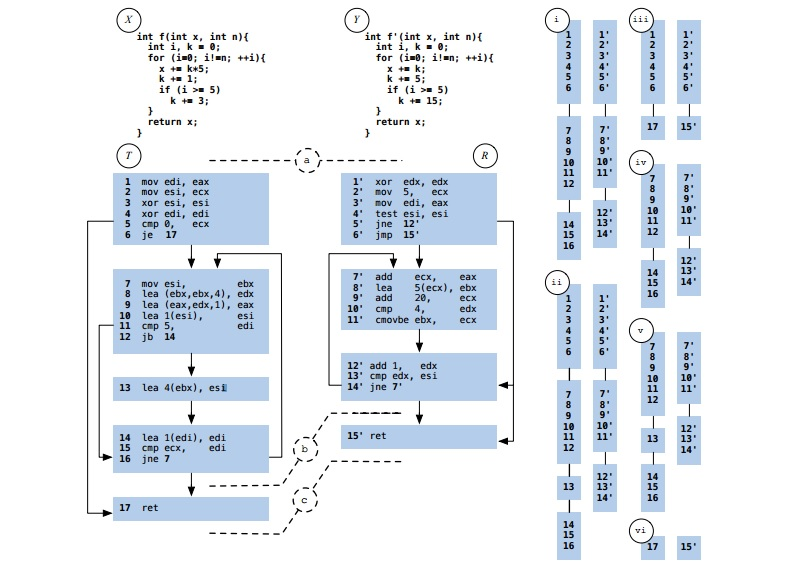
\includegraphics[width=15cm]{graf1.jpg}
		\end{center}
		\caption{Preverjanje ekvivalence med izvirnim in optimiziranim programom. Točke \texttt{a}, \texttt{b}, \texttt{c} označujejo lokacije rezanja. \texttt{i-vi} označujejo sekvenco izvajanje kode za vsako izmed trazicij}
		\label{pic1}
	\end{figure}
	
	V primeru programa na sliki \ref{pic1} sekvenci \texttt{i} in \texttt{ii} pripadata tranziciji iz \texttt{a} v \texttt{b}, sekvenca \texttt{iii} pripada tranziciji iz \texttt{a} v \texttt{c}, sekvenci \texttt{iv} in \texttt{v} pripadata tranziciji iz \texttt{b} v \texttt{b} in sekvenca \texttt{vi} pripada tranziciji iz \texttt{b} v \texttt{c}. Problem, ki se pojavi med izvajanjem je, kakšne invarjante mora točka \texttt{b} imeti, da bi statistično dokazal, da izvajanje zaporedja $R$ sledi izvajanju ustreznemu zaporedju programa $T$ in da izvajanje obeh programov gre skozi enake koščke. Rešitev takega problema se najbe v analizi podatkov. Program indentificira pot z ujemanjem sledi obeh zank na enakem vhodu podatkov na množici točk rezanj. Za pogoje relacije pri točki \texttt{b} lahko program preveri vrednosti živih registrov dobljene pri izvajanju obeh programov. Pri tem pridobi matrico, v kateri prva vrstica vsebuje vrednosti registrov, ko prvič doseže točko \texttt{b} in druga vrstica vsebuje vrednosti, ko drugič doseže točko \texttt{b}. Iz tega lahko izvleče relacijo med vrednosti s pomočjo linearne algebre tako, da izračuna ničelni prostor matrice s pomočjo knjižnice Integer Matrix Library. Tak algoritem predpostavlja, da koda vsebuje le eno zanko, vendar je to možno trivialno razširiti na primere z več zank in z notranjimi zankami tako, da za vsak kos kode ponovno izvedemo rezanje. V algoritmu je tudo možno razširiti monžico invarjant, tako da določimo največjo stopnjo monoma in dodamo vse monome, ki so manjše od the stopnje. Ker lahko ne-linearen invarianta predstalja disjunkcijo linearnih enkakovrednosti, je lahko tudi v množici invarjant vsebovana tudi določeno število disjunktivnih izrazov enakovrednosti. Disjuktni izraze rešuje z že obstoječim algoritmom Z3 \cite{article3}. Pri računanju živih registrov DDEC upošteva, da na 64 bitnih x86 arhitekturah za nekatere registre obstaja množica imenov. Vsako ima naslavja en del registra (Npr. prvih 8, 16, 32 bitov). Kadar ukaz zahteva pisannje v en del reistra, program označi cel rigister kot živega. Da lahko program opazuje vrednosti živih registrov pri točkah rezanja, se zanaša na sposobnost opazovanja ciljne lokacje in dinamično spreminjanje vrednosti s pomočjo zbirnika JIT. Pred izvajanjem optimizacije, DDEC rezervira del pomnilnika. Pri izvajanju vsakega ukaza optimizator pošlje signal za klic funkcije \texttt{record()}, ki shrani stanje naprave in vrednosti, ki so bile prebrane ali napisane v pomnilniku. Ko se izvajanje ciljne funkcije konča, tabela sledov vsebuje vse zapise manipulacije vrednosti na registrih in pomnilniku. Problem lahko nastane, da nekateri kandidati za ponovn zapis lahko kažejo na neveljano lokacijo v pomnilniku. Rešitev je se skriva v funkciji \texttt{sandbox()}. Pri izvajanju programa program pridobi največje velikost alociranih podatkov v pomnilniku in minimalen in maksimalen naslov v pomnilniku. Pridobljene vrednosti uporabi za rezervacijo drugega dela pomnilnika, da zavaruje izvajanje optimiziranega programa. Velikost podatkov rezervirenega pomnilnika ne presega velikosti rezerviranega izvirnega programa. Kazalci na pomnilniško mesto so zavarovano z funkcijo \texttt{sandbox\_addr()}, ki poskrbi da dostop do pomnilnika znotraj meja in blokira vse vstale dostope in ob primeru blokade ustavi izvajanje. Če je potrebno, lahko delež rezerviranega pominilnika povečamo. Poleg tega se optimizator zavaruje pred nastalimi neskončnimi zankami s klicom \texttt{sandbox\_jump}, ki prešteje kolikokrat je program skočil nazaj in prekine izvajanje, če preseže maksimalno število skokov nazaj. Program mora še poskrbeti, da se konča z ukazov za vrnitev na mesto izvajanje pred klicem, le če so invarjante izpolnjene. Za to poskrbi funkcija \texttt{sanbox\_return()}. Zaradi strukture in načina delovanja, algoritem dopušča uporabo še za reševanje drugih težav (Npr. avtomatično učenje množice ukazov glede na podano osnovno množico \cite{article4}).%
	%
		\begin{figure}[htb]
			\begin{center}
				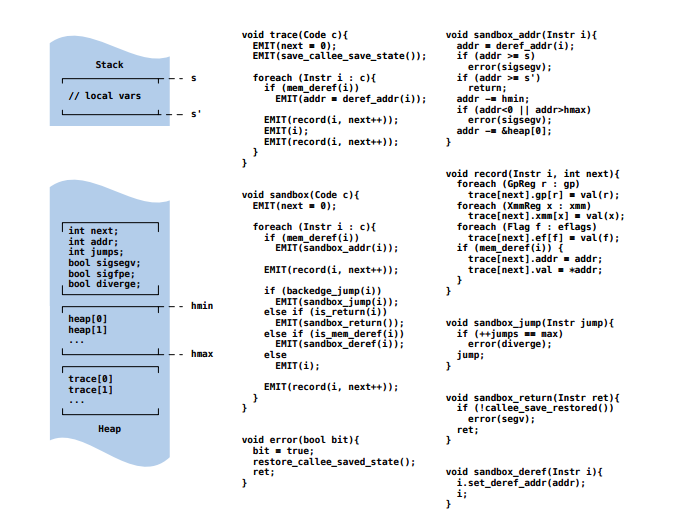
\includegraphics[width=15cm]{graf3.jpg}
			\end{center}
			\caption{Implementacija za sledenje izvajanje programov in izpisanih programov s pomočjo JIT zbirnika}
			\label{pic3}
		\end{figure}
	%
	STOKE trenutno vsebuje 8 transformacij. Prva transformacija se imenuje \texttt{add\_nops}. Transformacija doda \texttt{nop} ukaz, ki ne naredi ničesar. Naslednja tranformacija je \text{delete}, ki odstrani en ukaz. Potem je transformacija \texttt{instruction}, ki zamenja instrukcijo z drugo naključno. Poleg zamenjave instrukcije obstaja transformacija \texttt{opcode} in \texttt{operand}, ki zamenjata le operacijsko kodo oz. operand. Naslednja se imenuje \texttt{rotate}, ki vzame en ukaz iz segmenta in ga doda drugemu segmentu, ne da bi spremenil zaporedje ostalih ukazov. Potem ob obstajata texttt{local\_swap} in texttt{global\_swap}, ki zamenjata dva ukaza med seboj. Rezlika je v tem, da sta ukaza, ki ju menjamo, v istem segmentu, v druigi pa nista. Transformacije dovoljujejo, da so lahko neuspešne.%
	%
	\begin{figure}[htb]
		\begin{center}
			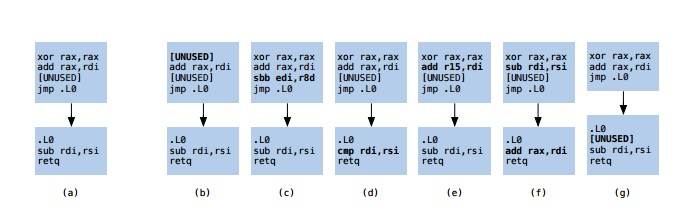
\includegraphics[width=13.5cm]{graf2.jpg}
		\end{center}
		\caption{Grafični pregled transformacij. Vsaka izmed primerov predstavlja tranformacijo: a) trenutni program, b) \texttt{delete}, c) \texttt{instruction}, d) \texttt{opcode}, e) \texttt{operand}, f) \texttt{global\_swap}, g) \texttt{resize}. Unused lahko zamenjamo z ukazom \texttt{nop}}
		\label{pic2}
	\end{figure}
	%
	STOKE ima plementiran algoritem za optimizacijo računanja s števili s plavajočo vejico. Kot je v ploglavju \ref{fl} omenjeno, optimizacija števil s plavojočo vejico ni preprosta, saj je v registrih in pomnilnikih shranjena zaokrožena vrednost, ki je najbližji napisani vrednosti v izvirni kodi. Še bolj se dejstvo zakomplicira, ko upoštevamo, da se med vsako operacijo število zaokrožuje \cite{float2}. Zato je v optimizatorju implementiran algoritem, ki preverja odstopanje med izvirnim in dobljenim programom. Pri računanju odstopanja pa se pojavi problem. Najbolj razširjena načina za računanje odstopa, sta relativna in absolutna razlika. Absolutno razliko dobimo tako, da iz dobljene vrenosti odštejemo prvotno vrednost. Če pa abolutno razliko delimo z prvotno vrednostjo, dobimo relativno vrednost. Oba načina imata problem pri računanju odstopanja. Absolutna razlika se v večjimi števili povečuje, Relativna vrednost, pa se povečuje pri denomlaliziranih številih. Tak problem se še bolj povečuje z računanjem ne-sosednjih števil. Zato je za izračun odstopanja uporabljen algoritem negotovost v zadnjem mestu (uncertainty in the last place), ki izmeri razliko med realnim številom in najbližjim predstavljen številu s plavojoćčo vejico v registru. V tem primeru STOKE računa razliko med stare in nove vrednosti v registru v ciljnem programu. Prednost take funkcije je, da lahko razliko izračuna tudi, če je kot argment podan noskončno ali nedefinirano število. ULP v C-ju potrebuje dva argumenta tipa \texttt{double}. Funkcija najprej predefinira ragumente, tako da vrednost shranjena v spremenljivki prebere kot celoštevilsko vrednost in vrne absolutno razliko med argumentoma. Pri tem še popravi porazdelitev števila s plavajočo vejico od minus neskončno do 0 tako da od celoštevilske vrednosti odšteje minimalno možno vrednost, ki jo lahko celoštevilska vrednost zavzeme, saj prvotno bi najmanjša vrednost predstavljala negativno ničlo in 0 bi prestavljala negativno nedefinirano število. Skupno odstopanje med izvirnim in dobljenim programom izračuna tako, da vzeme maksimalno odstopanje enega podatka, saj s tem prepreči možnost preliva pri seštevanju takih števil. STOKE sprejme končen program v primeru, če ne odstopa za več kot \(n\), ki je določena s strani uporabnika.
	
	\subsection{Zagon}
	\label{zg1}
	Kot je že omenjeno v \ref{lab1}, za zagon potrebujemo linux sistem (najprimernejši Ubuntu 14.02). Zraven še moramo imeti nameščenih nekaj knjižnjic in programov. Vse potrebne programe lahko namestimo s pomočjo ukaza \texttt{apt-get} v ukazni vrstici. Pri tem še moramo preveriti, če je gcc prevajalnik (C prevajalnik) in g++ (C++ prevajalnik) verzije 4.9, sicer prevajalnika ne bomo mogli sestaviti. Najprej moramo s pomočjo \texttt{git} ukaza prenesti datoteke z repozitorija.
	\medskip
		
	\noindent
	{\it Git ukaz:}
\begin{Verbatim}[baselinestretch=1]
git clone https://github.com/StanfordPL/stoke
\end{Verbatim}

	Ko je prenos končan, moramo nastaviti konfiguracijo za prevajanje optimizatorja v delujoč program. V glavni mapi stoke je skripta, ki nam to avtomatsko naredi, nato poženemo datoteko Makefile.
	\medskip
	
	\noindent
	{\it Zaporedje ukazov v ukazni vrstici:}
	\begin{Verbatim}[baselinestretch=1]
./configure.sh
make
	\end{Verbatim}
	
	Datoteka Makefile bo poskrbela za vse konfiguracije in prevajanje programov. Da lahko program poženemo iz kateregakoli direktorija moramo nastaviti globalno spremenljivko \texttt{PATH} v operacijskem sistemu.
	\medskip
	
	\noindent
	{\it Ukaz v ukazni vrstici:}
	\begin{Verbatim}[baselinestretch=1]
export PATH=$PATH:/<pot_do_stoke>/bin
	\end{Verbatim}
	
	\noindent
	{\small (\texttt{<pot\_do\_stoke>} predstavlja direktorij, ki se nahaja v mapi stoke)}
	
	Pred zagonom potrebujemo že posebej preveden program. Optimizator poženemo z ukazno vrstico. Pri tem moramo podati argumente. Argumente lahko podamo na dva načina. Prvi način je, da podamo argumente v ukazni vrstici. Drugi način je, da podamo datoteko ki ima v njej zapisane argumente. 
	\medskip
	
	\noindent
	{\it Primer ukaza v ukazni vrstici za prvi način:}
\begin{Verbatim}[baselinestretch=1]
stoke extract -i ./a.out -o bins
\end{Verbatim}
\medskip

\noindent
{\it Primer ukaza v ukazni vrstici za drugi način:}
\begin{Verbatim}[baselinestretch=1]
stoke extract --config extract.conf
\end{Verbatim}
\medskip

\noindent
{\it Primer datoteke extract.conf:}
\begin{Verbatim}[baselinestretch=1]
-i ./a.out  # Lokacija in ime datoteke, ki želimo optimizirati
-o bins     # Lokacija kjer shrani izvlečeno kodo
\end{Verbatim}
\noindent
{\small (Zank \texttt{\#} označuje kdaj se komentar v vrstici začne.)} 

\medskip

\noindent
{\it Primer kode, ki jo bomo obdelali:}
\begin{Verbatim}[baselinestretch=1]
#include <cstdlib>
#include <stddef.h>
#include <stdint.h>

using namespace std;

size_t popcnt(uint64_t x) {
	int res = 0;
	for ( ; x > 0; x >>= 1 ) {
		res += x & 0x1ull;
	}
	return res;
}

int main(int argc, char** argv) {
	const auto itr = atoi(argv[1]);

	auto ret = 0;
	for ( auto i = 0; i < itr; ++i ) {
		ret += popcnt(i);
	}

	return ret;
}
\end{Verbatim}
\noindent
{\small (Koda poišče vse bite, ki vsebujejo vrednost 1 od števila 0 do \texttt{itr} v bitni reprezentaciji, kjer \texttt{itr} podan kot prvi argument.)}

Potem moramo generirati nekaj poskusnih primerov za določeno funkcijo. Ti primeri bodo uporabljeni za preverjanje pravilnosti kode. Funkcije najdene v programu imajo drugačna imena kot v izvirni kodi, zato je potrebno pogledati v mapi, kjer je bila izvlečena koda, kako se imenuje. Ponavadi je ime funkcije v izvirni kodi vsebovana v imenu datoteke.

\medskip

\noindent
{\it Primer ukaza:}
\begin{Verbatim}[baselinestretch=1]
stoke testcase --config testcase.conf
\end{Verbatim}
\medskip

\noindent
{\it Primer izgleda datoteke testcase.conf:}
\begin{Verbatim}[baselinestretch=1]
--bin ./a.out        # Lokacija in ima datoteke prevedenega programa
--args 10000000      # Argument, ki so podani za ./a.out
--functions bins     # Lokacija, kjer je shranjena izvlečena funkcija

-o popcnt.tc         # Pot do datoteke kjer naj shrani poskusne teste

--fxn _Z6popcntm     # Ime funkcije, za katerega naredi poskusne teste
--max_testcases 1024 # Maximalno število testov.
\end{Verbatim}
\medskip

\noindent
{\it Primer datoteke \_Z6popcntm:}
\begin{Verbatim}[baselinestretch=1]
.text
.globl _Z6popcntm
.type _Z6popcntm, @function #ime funkcije

#! file-offset 0x580
#! rip-offset  0x400580
#! capacity    48 bytes

# Text            #  Line  RIP       Bytes  Opcode             
._Z6popcntm:      #        0x400580  0      OPC=<label>        
testq %rdi, %rdi  #  1     0x400580  3      OPC=testq_r64_r64  
je .L_40059f      #  2     0x400583  2      OPC=je_label       
xorl %eax, %eax   #  3     0x400585  2      OPC=xorl_r32_r32   
nop               #  4     0x400587  1      OPC=nop            
nop               #  5     0x400588  1      OPC=nop                       
.L_400590:        #        0x400590  0      OPC=<label>        
movl %edi, %edx   #  13    0x400590  2      OPC=movl_r32_r32   
andl $0x1, %edx   #  14    0x400592  3      OPC=andl_r32_imm8  
addl %edx, %eax   #  15    0x400595  2      OPC=addl_r32_r32   
shrq $0x1, %rdi   #  16    0x400597  3      OPC=shrq_r64_one   
jne .L_400590     #  17    0x40059a  2      OPC=jne_label      
cltq              #  18    0x40059c  2      OPC=cltq           
retq              #  19    0x40059e  1      OPC=retq           
.L_40059f:        #        0x40059f  0      OPC=<label>        
xorl %eax, %eax   #  20    0x40059f  2      OPC=xorl_r32_r32   
retq              #  21    0x4005a1  1      OPC=retq           
nop               #  22    0x4005a2  1      OPC=nop                      

.size _Z6popcntm, .-_Z6popcntm
\end{Verbatim}
\noindent
{\small (Zank \texttt{\#} označuje kdaj se komentar v vrstici začne. Zgoraj navedena datoteka je skrajšana. Vsi manjkajoči ukazi so ukazi, ki ne naredijo ničesar)}

V datoteki (v tem primeru popcnt.tc) je izpisano stanje programa pred vstopom v funkcijo. Prvih 60 vrstic označuje stanje vseh registrov. Naslednjih nekaj vrstic opisuje stanje v delu pomnilnika, kjer se nahajajo kazalci za delovanje programa.

 \medskip
 
 \noindent
 {\it Primer datoteke \_Z6popcntm:}
 \begin{Verbatim}[baselinestretch=1]
Testcase 0:
 
%rax     00 00 00 00 00 98 96 80
%rcx     00 00 00 00 00 00 00 00
%rdx     00 00 00 00 00 00 00 0a
%rbx     00 00 00 00 00 00 00 01
%rsp     00 00 7f ff 97 44 36 28
%rbp     00 00 00 00 00 00 00 00
%rsi     19 99 99 99 99 99 99 99
%rdi     00 00 00 00 00 00 00 00
%r8      00 00 2a c9 68 1a 50 40
%r9      00 00 7f ff 97 44 46 01
%r10     00 00 00 00 00 98 96 80
%r11     00 00 00 00 00 00 00 0a
%r12     00 00 00 00 00 98 96 80
%r13     00 00 7f ff 97 44 37 20
%r14     00 00 00 00 00 00 00 00
%r15     00 00 00 00 00 00 00 00

%ymm0    00 00 00 00 00 00 00 00 00 00 00 00 00 00 00 00 
		 00 00 00 00 00 00 00 00 00 00 00 00 00 ff 00 00
%ymm1    00 00 00 00 00 00 00 00 00 00 00 00 00 00 00 00 
         2f 2f 2f 2f 2f 2f 2f 2f 2f 2f 2f 2f 2f 2f 2f 2f
%ymm2    00 00 00 00 00 00 00 00 00 00 00 00 00 00 00 00 
	     00 00 00 00 00 00 00 00 00 00 00 00 00 00 00 00
%ymm3    00 00 00 00 00 00 00 00 00 00 00 00 00 00 00 00 
	   	 00 00 00 00 00 00 00 ff 00 00 00 00 00 00 00 ff
%ymm4    00 00 00 00 00 00 00 00 00 00 00 00 00 00 00 00 
         00 00 00 00 00 00 00 00 00 00 00 00 00 00 00 00
%ymm5    00 00 00 00 00 00 00 00 00 00 00 00 00 00 00 00 
         00 00 00 00 00 00 00 00 00 00 00 00 00 00 00 00
%ymm6    00 00 00 00 00 00 00 00 00 00 00 00 00 00 00 00 
         00 00 00 00 00 00 00 00 00 00 00 00 00 00 00 00
%ymm7    00 00 00 00 00 00 00 00 00 00 00 00 00 00 00 00 
         00 00 00 00 00 00 00 00 00 00 00 00 00 00 00 00
%ymm8    00 00 00 00 00 00 00 00 00 00 00 00 00 00 00 00 
         00 00 00 00 00 00 00 00 00 00 00 00 00 00 00 00
%ymm9    00 00 00 00 00 00 00 00 00 00 00 00 00 00 00 00 
         00 00 00 00 00 00 00 00 00 00 00 00 00 00 00 00
%ymm10   00 00 00 00 00 00 00 00 00 00 00 00 00 00 00 00 
         00 00 00 00 00 00 00 00 00 00 00 00 00 00 00 00
%ymm11   00 00 00 00 00 00 00 00 00 00 00 00 00 00 00 00 
         00 00 00 00 00 00 00 00 00 00 00 00 00 00 00 00
%ymm12   00 00 00 00 00 00 00 00 00 00 00 00 00 00 00 00 
         00 00 00 00 00 00 00 00 00 00 00 00 00 00 00 00
%ymm13   00 00 00 00 00 00 00 00 00 00 00 00 00 00 00 00 
         00 00 00 00 00 00 00 00 00 00 00 00 00 00 00 00
%ymm14   00 00 00 00 00 00 00 00 00 00 00 00 00 00 00 00 
         00 00 00 00 00 00 00 00 00 00 00 00 00 00 00 00
%ymm15   00 00 00 00 00 00 00 00 00 00 00 00 00 00 00 00 
         00 00 00 00 00 00 00 00 00 00 00 00 00 00 00 00
 
%cf      0 
%1       1 
%pf      1 
%0       0 
%af      0 
%0       0 
%zf      0 
%sf      0 
%tf      0 
%if      1 
%df      0 
%of      0 
%iopl[0] 0 
%iopl[1] 0 
%nt      0 
%0       0 
%rf      0 
%vm      0 
%ac      0 
%vif     0 
%vip     0 
%id      0 
 
 [ 00007fff 97443630 - 00007fff 97443620 ]
 [ 1 valid rows shown ]
 
 00007fff 97443628   d d d d d d d d   00 00 00 00 00 40 04 6c
 
 [ 00000000 00000000 - 00000000 00000000 ]
 [ 0 valid rows shown ]
 
 [ 00000000 00000000 - 00000000 00000000 ]
 [ 0 valid rows shown ]
 
 0 more segment(s)
 \end{Verbatim}
 \noindent
 {\small (registri \%ymm od 0 do 15 so v datoteki napisani vse v eni vrstici. Tukaj so napisani v dveh zaradi preglednosti.)}

Šele zdaj lahko poženemo optimiziranje. Pri tem še moramo upošteviti, da različne kode lahko zahtevajo različno konfiguracijo. Paziti moramo na to, kateri registri so definirani pred vhodom v funkcijo in kateri registri so definirani ob izhodu iz funkcije. Pozorni moramo biti tudi na število iteracij za ponovni začetek in na maksimalno število iteracij. Večji programi potrebujejo večjo število iteracij za optimizacijo kot manjši programi. 

\medskip

\noindent
{\it Primer ukaza:}
\begin{Verbatim}[baselinestretch=1]
stoke synthesize --config synthesize.conf
\end{Verbatim}
\medskip

\noindent
{\it Primer izgleda datoteke testcase.conf:}
\begin{Verbatim}[baselinestretch=1]
--out result.s               # Pot kjer naj napiše rezultat

--target bins/_Z6popcntm.s   # Pot do funkcije za optimizacijo

--def_in "{ %rax %rdi }"     # Registri ki so živi na začetku
--live_out "{ %rax }"        # Registri ki so živi na koncu

--testcases popcnt.tc        # Datoteka z poskusnimi testi
--training_set "{ 0 ... 7 }" # Testi za merjenje pravilnosti med iskanjem
--test_set "{ 8 ... 1023 }"  # Testi za preverjanje pravilnosti

--distance hamming           # Način za merejenje napak za izhodne ragistre
--misalign_penalty 1         # Kazen za razultate, ki se nahajajo 
                             # na napačnem mestu
--reduction sum              # Metoda za izračun nepravilnosti
--sig_penalty 9999           # Točke za rezultat, ki povzročijo neničelne 
                             # signale 

--cost "correctness + latency" # Način izračuna izvedbe

--global_swap_mass 0         # Nastavitev cene
--instruction_mass 1         # Nastavitev cene
--local_swap_mass 1          # Nastavitev cene
--opcode_mass 1              # Nastavitev cene
--operand_mass 1             # Nastavitev cene
--rotate_mass 0              # Nastavitev cene

--beta 1                       # Konstanta za izračun sprejemljivosti
--initial_instruction_number 5 # Število nop operacij

--statistics_interval 100000  # Printanje statistike na vsakih n iteracij
--timeout_iterations 16000000 # Nastavitev število operacij preden konča
--cycle_timeout 1000000       # Ponovni začetek vsakih n iteracij

--strategy hold_out           # Določa strategijo preverjanje
\end{Verbatim}

Po končanem optimiziranju, optimizator napiše optimizirano kodo v datoteko, podano kot argument. Optimizator ima možnost, da optimizirano kodo vstavi nazaj v že preveden program. 

\medskip

\noindent
{\it Primer ukaza:}
\begin{Verbatim}[baselinestretch=1]
stoke replace --config replace.conf
\end{Verbatim}
\medskip

\noindent
{\it Primer izgleda datoteke replace.conf:}
\begin{Verbatim}[baselinestretch=1]
-i ./a.out         # Pot do prevedenega programa
--rewrite result.s # Pot do optimizirane funkcije
\end{Verbatim}
\section{Primeri optimizacije}
\label{priG2}
Tukaj je nekaj delov programa, ki jih je optimizator optimiziral in njihov pripadajoči optimiziran program. Testiranje deluje v dveh delih. Prvi del je optimiziranje kratkih programov (enakih kot v \ref{priG}), drugi del pa vsebuje poskuse na večjih programih. Taka delitev nam bo dala vpogled, kako dobro se je STOKE odrezal v primerjavi z GNU-Superoptimizer, pa čeprav pri GNU-Superoptimizer-ju nimamo rezultatov za večje programe.  
\subsection{Optimizacija krajših programov}
Ko je že omenjeno v poglavju \ref{priG2}, v tem poglavju so rezultati optimizacij krajših programov. Vsi primeri kod so enaki kot v točki \ref{priG}. Prvi primer optimizacije je funkcija, ki izračuna absolutno vrednost nekega števila. 
\medskip

\noindent
{\it Primer dela kode:}
\begin{Verbatim}[baselinestretch=1]
return (v0 < 0 ? -v0 : v0);
\end{Verbatim}

Optimizator je poskušal najti optimalno kodo. To je naslednji rezultat. 
\medskip

\noindent
{\it Predlagana rešitev:}
\begin{Verbatim}[baselinestretch=1]
.text
.globl _Z5abss2l
.type _Z5abss2l, @function

#! file-offset 0x690
#! rip-offset  0x400690
#! capacity    32 bytes

# Text            #  Line  RIP       Bytes  Opcode             
._Z5abss2l:       #        0x400690  0      OPC=<label>        
movq %rdi, %rdx   #  1     0x400690  3      OPC=movq_r64_r64   
movq %rdi, %rax   #  2     0x400693  3      OPC=movq_r64_r64   
sarq $0x3f, %rdx  #  3     0x400696  4      OPC=sarq_r64_imm8  
xorq %rdx, %rax   #  4     0x40069a  3      OPC=xorq_r64_r64   
subq %rdx, %rax   #  5     0x40069d  3      OPC=subq_r64_r64   
retq              #  6     0x4006a0  1      OPC=retq           
nop               #  7     0x4006a1  1      OPC=nop                       

.size _Z5abss2l, .-_Z5abss2l
\end{Verbatim}

Za naslednji test je optimizator iskal rešitev za enako funkcijonalnost, kot v prejšnjem testu, vendar koda je drugače napisana. Pri tej kodi manjka \texttt{else} stavek.
\medskip

\noindent
{\it Primer Drugačne napisane kode:}
\begin{Verbatim}[baselinestretch=1]
if(x<0){x=-x;}
return x;
\end{Verbatim}

Za ta test je optimizator dobil enak rezultat kot pri prejšnjem testu.

\medskip

\noindent
{\it Ena izmed rešitev:}
\begin{Verbatim}[baselinestretch=1]
.text
.globl _Z4abssl
.type _Z4abssl, @function

#! file-offset 0x640
#! rip-offset  0x400640
#! capacity    32 bytes

# Text            #  Line  RIP       Bytes  Opcode             
._Z4abssl:        #        0x400640  0      OPC=<label>        
movq %rdi, %rdx   #  1     0x400640  3      OPC=movq_r64_r64   
movq %rdi, %rax   #  2     0x400643  3      OPC=movq_r64_r64   
sarq $0x3f, %rdx  #  3     0x400646  4      OPC=sarq_r64_imm8  
xorq %rdx, %rax   #  4     0x40064a  3      OPC=xorq_r64_r64   
subq %rdx, %rax   #  5     0x40064d  3      OPC=subq_r64_r64   
retq              #  6     0x400650  1      OPC=retq           
nop               #  7     0x400651  1      OPC=nop                        

.size _Z4abssl, .-_Z4abssl
\end{Verbatim}

Za naslednji test je bila podana funkcija, ki pove če je število manjše, večje ali enako številu 0. Pri tem je bila uporabljena naslednja koda.
\medskip

\noindent
{\it Primer kode:}
\begin{Verbatim}[baselinestretch=1]
return (v0 > 0 ? 1 : (v0 < 0 ? -1 : 0));
\end{Verbatim}

Za ta test lahko opazimo, da optimizator ne obide nekaterih pogojnih skokov, ki bi jih sicer lahko obšli.
\medskip

\noindent
{\it Ena izmed rešitev:}
\begin{Verbatim}[baselinestretch=1]
  .text
  .globl _Z4sgn2l
  .type _Z4sgn2l, @function
  
  #! file-offset 0x6b0
  #! rip-offset  0x4006b0
  #! capacity    32 bytes
  
  # Text            #  Line  RIP       Bytes  Opcode              
  ._Z4sgn2l:        #        0x4006b0  0      OPC=<label>         
  cmpq $0x0, %rdi   #  1     0x4006b0  4      OPC=cmpq_r64_imm8   
  movl $0x1, %eax   #  2     0x4006b4  5      OPC=movl_r32_imm32  
  jle .L_4006c0     #  3     0x4006b9  2      OPC=jle_label       
  retq              #  4     0x4006bb  1      OPC=retq            
  nop               #  5     0x4006bc  1      OPC=nop             
  .L_4006c0:        #        0x4006c0  0      OPC=<label>         
  setne %al         #  9     0x4006c0  3      OPC=setne_r8        
  movzbl %al, %eax  #  10    0x4006c3  3      OPC=movzbl_r32_r8   
  negq %rax         #  11    0x4006c6  3      OPC=negq_r64        
  retq              #  12    0x4006c9  1      OPC=retq            
  nop               #  13    0x4006ca  1      OPC=nop                          
  
  .size _Z4sgn2l, .-_Z4sgn2l
\end{Verbatim}

Za naslednji test je bila uporabljena funkcija z enako funkcijonalnostjo kot pri prejšnjem testu. Koda tokrat uporablja \texttt{else if} stavek in za vsak izpolnjen pogoj, takoj vrne rešitev.
\medskip

\noindent
{\it Primer drugače zapisane kode:}
\begin{Verbatim}[baselinestretch=1]
if(x<0){return 1;}
else if(x>0){return -1;}
else{return 0;}
\end{Verbatim}
Ta poskus ni prinesel nobenih sprememb.
\medskip

\noindent
{\it Ena izmed rešitev:}
\begin{Verbatim}[baselinestretch=1]
  .text
  .globl _Z3sgnl
  .type _Z3sgnl, @function
  
  #! file-offset 0x660
  #! rip-offset  0x400660
  #! capacity    32 bytes
  
  # Text            #  Line  RIP       Bytes  Opcode              
  ._Z3sgnl:         #        0x400660  0      OPC=<label>         
  cmpq $0x0, %rdi   #  1     0x400660  4      OPC=cmpq_r64_imm8   
  movl $0x1, %eax   #  2     0x400664  5      OPC=movl_r32_imm32  
  jle .L_400670     #  3     0x400669  2      OPC=jle_label       
  retq              #  4     0x40066b  1      OPC=retq            
  nop               #  5     0x40066c  1      OPC=nop                     
  .L_400670:        #        0x400670  0      OPC=<label>         
  setne %al         #  9     0x400670  3      OPC=setne_r8        
  movzbl %al, %eax  #  10    0x400673  3      OPC=movzbl_r32_r8   
  negq %rax         #  11    0x400676  3      OPC=negq_r64        
  retq              #  12    0x400679  1      OPC=retq            
  nop               #  13    0x40067a  1      OPC=nop                         
  
  .size _Z3sgnl, .-_Z3sgnl
\end{Verbatim}

Naslednji podan primer nastavi 0, če je število večje ali enako 0, drugače 1.
\medskip

\noindent
{\it Primer kode:}
\begin{Verbatim}[baselinestretch=1]
return v0 <= 0;
\end{Verbatim}
Optimizator najde optimalno kodo dolžine 3 inštrukcije, brez upoštevanja zadnjega \texttt{retq} ukaza, ki je ukaz za vrnitev na zadnji izveden ukaz na prejšnji funkciji.
\medskip

\noindent
{\it Ena izmed rešitev:}
\begin{Verbatim}[baselinestretch=1]
  .text
  .globl _Z4lte2l
  .type _Z4lte2l, @function
  
  #! file-offset 0x6d0
  #! rip-offset  0x4006d0
  #! capacity    16 bytes
  
  # Text            #  Line  RIP       Bytes  Opcode             
  ._Z4lte2l:        #        0x4006d0  0      OPC=<label>        
  xorl %eax, %eax   #  1     0x4006d0  2      OPC=xorl_r32_r32   
  testq %rdi, %rdi  #  2     0x4006d2  3      OPC=testq_r64_r64  
  setle %al         #  3     0x4006d5  3      OPC=setle_r8       
  retq              #  4     0x4006d8  1      OPC=retq           
  nop               #  5     0x4006d9  1      OPC=nop                        
  
  .size _Z4lte2l, .-_Z4lte2l
\end{Verbatim}

Kot pri ostalih poskusih, je tudi za ta test narejena še ena poskusna koda, ki pa tokrat vrača vrednosti, takoj ko je eden izmed pogojev izpolnjen.

\medskip

\noindent
{\it Primer drugačne kode:}
\begin{Verbatim}[baselinestretch=1]
if(x<=0){return 1;}
else{return 0;}
\end{Verbatim}
Rezultat ne kaže na odvisnost, kako zapišemo kodo, zato je ostala enaka.
\medskip

\noindent
{\it Ena izmed rešitev:}
\begin{Verbatim}[baselinestretch=1]
  .text
  .globl _Z3ltel
  .type _Z3ltel, @function
  
  #! file-offset 0x680
  #! rip-offset  0x400680
  #! capacity    16 bytes
  
  # Text            #  Line  RIP       Bytes  Opcode             
  ._Z3ltel:         #        0x400680  0      OPC=<label>        
  xorl %eax, %eax   #  1     0x400680  2      OPC=xorl_r32_r32   
  testq %rdi, %rdi  #  2     0x400682  3      OPC=testq_r64_r64  
  setle %al         #  3     0x400685  3      OPC=setle_r8       
  retq              #  4     0x400688  1      OPC=retq           
  nop               #  5     0x400689  1      OPC=nop                      
  
  .size _Z3ltel, .-_Z3ltel
\end{Verbatim}
\subsection{Optimizacija daljših programov}

V tem poglavju so rezultati optimizacij daljših in bolj kompleksnih programov. Ti programi so bili optimizirani večkrat z različnimi konfiguracijami. Razlog za takšen način testiranja je, da ugotovimo koliko časa se splača optimizirati nek program. Načrt je bil, da naprej izmerimo čas optimizacije programa, potem pa preverimo pravilnost optimiziranega programa in hitrost njegovega delovanja. Kljub temu pa načrt ni bil uspešen, saj so se pojavile nepravilnosti v optimiziranem programu. Razlog za nepravilnosti je lahko več. Prvi razlog je napačna konfiguracija optimizatorja med procesom optimiziranja. Pri vsaki funkciji moramo podati drugačno konfigurirajo. Kljub velikemu času posvečenem iskanju, je bilo neuspešno. Drugi problem je, da je sam optimizator nestabilen. Optimizator poskuša uporabljati ukaze za katere ni podprto validacijo. Zaradi tega ostaja možnost, da je iskanje povsem neuspešno. 

\section{Prednosti in slabosti}

Kot vsi optimizatorji ima tudi ta optimizator nekaj prednosti in slabosti. Prva prednost takega optimizatorja je, da lahko uporablja bolj kompleksne ukaze (npr. \texttt{popcnt}). Druga prednost je način iskanja optimizacija nekega programa. Optimizator ima veliko različnih konfiguracij in načinov iskanja. Uporabnik lahko izbira med gradnjo kode ali optimizacijo prejšnje kode, strategijo načina iskanja. Dodatna vrednost je še v tem, da ima optimizator ločene dele programov, ki lahko spreminjamo in dodajamo ne da bi ogrozili ostale module. Slaba stvar takega optimizatorja je, da uporabnik so mora spoznati na arhitekturo procesorja in na zbirno kodo, ki ga ta procesor uporablja. Pri tem še mora vedeti, kako nastaviti konfiguracijo za iskanje, kar je za preprostega uporabnika preprosto preveč. Poleg tega je še potrben človeški vnos skozi cel postopek optimiziranja. Najšlabše dejstvo pa je, da ta optimizator ni stabilen, saj potrebuje točno določen prevajalnik, točno določen operacijski sistem in ima še vedno težave pri prevajanju in zagonu optimizatorja. Superoptimizator je bolj uporaben za optimizacijo manjših funkcij v programu, saj lahko za celo vsebino funkcije zamenja z enim samim ukazom. Po vsaki optimizaciji moramo preveriti, če program deluje pravilno.

\chapter{GNU Compiler Collection}
\label{ch3}
GCC je napisal Richard Matthew Stallman leta 1987 kot prevajalnik za projekt GNU, tako da bi bil na voljo kot prosto programje. Njegov razvoj je večinoma vodila Free Software Foundation. Skupina razvijalcev, ki je bila nezadovoljna s počasnim napredovanjem in zaprto naravo uradnega razvoja GCC, je leta 1997 razvila projekt z imenom EGCS (Experimental/Enhanced GNU Compiler System). S projektom so povezali več preskusnih odcepljenih programih v posamezen projekt, izvirajoč iz GCC. Razvoj EGCS se je kasneje pokazal za precej bolj življenjskega od razvoja GCC, tako da so aprila 1999 končno določili kot uradno različico GCC. Sedaj GCC vzdržuje več skupin programerjev iz celega sveta. Prenesli so ga na več različnih vrst procesorjev in operacijskih sistemov kot kateri drugi prevajalnik. GCC velikokrat izberejo za razvoj programske opreme, ki se bo izvajala na različni strojni opremi. Razlike domačinskih prevajalnikov vodijo do težav v razvijajoči programski kodi, ki se naj bi pravilno prevedla na vseh prevajalnikih in v izdelanih skriptah, ki bodo tekle na vseh platformah. Z uporabo GCC je enak razčlenjevalni program za vse platforme, in če se koda prevede na enem sistemu, je večja verjetnost, da se bo prevedla tudi na drugem. V nekaterih primerih GCC naredi počasnejše izvršne programe kot drugi prevajalniki, vendar se ga zaradi prostosti in možnih manjših razvojnih stroškov splača uporabiti.
\section{Opis programa in načina delovanja}
\label{loi}
Kot že omenjeno v poglavju \ref{ch3} GCC je prevajalk, vzdrževan prek več skupin programerjev. Prevajalnik je preprost za uporabo. Zaženemo ga lahko le z enim samim ukazom v ukazni vrstici. Prevajanik privzeto ne optimizira kode, vendar ima nastavitve, ki lahko omogočijo določene optimizacije. Omogočimo jih lahko tako, da dodamo zastavice in glede na zastavice, ki smo jih dali, potem program med prevajanjem optimizira. Ko končanem prevajanju, program preprosto izpiše preveden program v datoteko, ki jo lahko poženemo kasneje. Ker je prevajalnik namenjen za širšo publiko, je tudi optimizator, pakiran z prevajalnikom, odprt širši publiki. 
\subsection{Način optimiziranja}
Kot je že omenjeno v poglavju \ref{loi}, GCC mora imeti podane zastavice, ki povedo katere optimizacije naj opravi za določen program \cite{gcc}. Čas prevajanja je odvisen od omogočenih optimizacij. Poleg zamenjav funkcijonalnih enakih kod, optimizator omogoča vstavljanje generirane kode funkcije namesto klica funkcije in eliminacijo if stavkov in zank, katerih pogoj ni nikoli izpolnjen (ali je vedno izpolnjen pri if stavku).   
\section{Primeri optimizacije}
\label{priG3}
Tukaj je nekaj delov programa, ki jih je optimizator optimiziral in njihov pripadajoči optimiziran program. Testiranje deluje v dveh delih. Prvi del je optimiziranje kratkih programov (enakih kot v \ref{priG}), drugi del pa vsebuje poskuse na večjih programih. Taka delitev nam bo dala vpogled, kako dobro se je GNU Compiler Colection odrezal v primerjavi z GNU-Superoptimizer, pa čeprav pri GNU-Superoptimizer-ju nimamo rezultatov za večje programe.
\subsection{Optimizacija krajših programov}
\label{rez}
Ko je že omenjeno v poglavju \ref{priG3}, v tem poglavju so rezultati optimizacij krajših programov. Vsi primeri kod so enaki kot v točki \ref{priG}. Prvi primer optimizacije je funkcija, ki izračuna absolutno vrednost nekega števila. 
\medskip

\noindent
{\it Primer dela kode:}
\begin{Verbatim}[baselinestretch=1]
return (v0 < 0 ? -v0 : v0);
\end{Verbatim}

Optimizator je poskušal najti optimalno kodo. To je naslednji rezultat. 
\medskip

\noindent
{\it Predlagana rešitev:}
\begin{Verbatim}[baselinestretch=1]
(gdb) Dump of assembler code for function _Z5abss2l:
0x0000000000400770 <+0>: 	mov    %rdi,%rdx
0x0000000000400773 <+3>: 	mov    %rdi,%rax
0x0000000000400776 <+6>: 	sar    $0x3f,%rdx
0x000000000040077a <+10>:	xor    %rdx,%rax
0x000000000040077d <+13>:	sub    %rdx,%rax
0x0000000000400780 <+16>:	retq 
\end{Verbatim}

Za naslednji test je optimizator iskal rešitev za enako funkcijonalnost, kot v prejšnjem testu, vendar koda je drugače napisana. Pri tej kodi manjka \texttt{else} stavek.
\medskip

\noindent
{\it Primer Drugačne napisane kode:}
\begin{Verbatim}[baselinestretch=1]
if(x<0){x=-x;}
return x;
\end{Verbatim}

Za ta test je optimizator dobil enak rezultat kot pri prejšnjem testu.

\medskip

\noindent
{\it Ena izmed rešitev:}
\begin{Verbatim}[baselinestretch=1]
(gdb) Dump of assembler code for function _Z4abssl:
0x0000000000400720 <+0>: 	mov    %rdi,%rdx
0x0000000000400723 <+3>: 	mov    %rdi,%rax
0x0000000000400726 <+6>: 	sar    $0x3f,%rdx
0x000000000040072a <+10>:	xor    %rdx,%rax
0x000000000040072d <+13>:	sub    %rdx,%rax
0x0000000000400730 <+16>:	retq   
\end{Verbatim}

Za naslednji test je bila podana funkcija, ki pove če je število manjše, večje ali enako številu 0. Pri tem je bila uporabljena naslednja koda.
\medskip

\noindent
{\it Primer kode:}
\begin{Verbatim}[baselinestretch=1]
return (v0 > 0 ? 1 : (v0 < 0 ? -1 : 0));
\end{Verbatim}

Za ta test lahko opazimo, da optimizator ne obide nekaterih pogojnih skokov, ki bi jih sicer lahko obšli.
\medskip

\noindent
{\it Ena izmed rešitev:}
\begin{Verbatim}[baselinestretch=1]
(gdb) Dump of assembler code for function _Z4sgn2l:
0x0000000000400790 <+0>: 	cmp    $0x0,%rdi
0x0000000000400794 <+4>: 	mov    $0x1,%eax
0x0000000000400799 <+9>: 	jle    0x4007a0 <_Z4sgn2l+16>
0x000000000040079b <+11>:	repz retq 
0x000000000040079d <+13>:	nopl   (%rax)
0x00000000004007a0 <+16>:	setne  %al
0x00000000004007a3 <+19>:	movzbl %al,%eax
0x00000000004007a6 <+22>:	neg    %rax
0x00000000004007a9 <+25>:	retq 
\end{Verbatim}

Za naslednji test je bila uporabljena funkcija z enako funkcijonalnostjo kot pri prejšnjem testu. Koda tokrat uporablja \texttt{else if} stavek in za vsak izpolnjen pogoj, takoj vrne rešitev.
\medskip

\noindent
{\it Primer drugače zapisane kode:}
\begin{Verbatim}[baselinestretch=1]
if(x<0){return 1;}
else if(x>0){return -1;}
else{return 0;}
\end{Verbatim}
Ta poskus ni prinesel nobenih sprememb.
\medskip

\noindent
{\it Ena izmed rešitev:}
\begin{Verbatim}[baselinestretch=1]
(gdb) Dump of assembler code for function _Z3sgnl:
0x0000000000400740 <+0>: 	cmp    $0x0,%rdi
0x0000000000400744 <+4>: 	mov    $0x1,%eax
0x0000000000400749 <+9>: 	jle    0x400750 <_Z3sgnl+16>
0x000000000040074b <+11>:	repz retq 
0x000000000040074d <+13>:	nopl   (%rax)
0x0000000000400750 <+16>:	setne  %al
0x0000000000400753 <+19>:	movzbl %al,%eax
0x0000000000400756 <+22>:	neg    %rax
0x0000000000400759 <+25>:	retq  
\end{Verbatim}

Neslednji podan primer nastavi 0, če je število večje ali enako 0, drugače 1.
\medskip

\noindent
{\it Primer kode:}
\begin{Verbatim}[baselinestretch=1]
return v0 <= 0;
\end{Verbatim}
Optimizator najde optimalno kodo dolžine 3 inštrukcije, brez upoštevanja zadnjega \texttt{retq} ukaza, ki je ukaz za vrnitev na zadnji izveden ukaz na prejšnji funkciji.
\medskip

\noindent
{\it Ena izmed rešitev:}
\begin{Verbatim}[baselinestretch=1]
(gdb) Dump of assembler code for function _Z4lte2l:
0x00000000004007b0 <+0>:	xor    %eax,%eax
0x00000000004007b2 <+2>:	test   %rdi,%rdi
0x00000000004007b5 <+5>:	setle  %al
0x00000000004007b8 <+8>:	retq 
\end{Verbatim}

Kot pri ostalih poskusih, je tudi za ta test narejena še ena poskusna koda, ki pa tokrat vrača vrednosti, takoj ko je eden izmed pogojev izpolnjen.

\medskip

\noindent
{\it Primer drugačne kode:}
\begin{Verbatim}[baselinestretch=1]
if(x<=0){return 1;}
else{return 0;}
\end{Verbatim}
Rezultat ne kaže na odvisnost, kako zapišemo kodo, zato je ostala enaka.
\medskip

\noindent
{\it Ena izmed rešitev:}
\begin{Verbatim}[baselinestretch=1]
(gdb) Dump of assembler code for function _Z3ltel:
0x0000000000400760 <+0>:	xor    %eax,%eax
0x0000000000400762 <+2>:	test   %rdi,%rdi
0x0000000000400765 <+5>:	setle  %al
0x0000000000400768 <+8>:	retq
\end{Verbatim}
\subsection{Optimizacija daljših programov}

V tem poglavju so rezultati optimizacij daljših in bolj kompleksnih programov. Ti programi so bili optimizirani večkrat z različnimi konfiguracijami. Razlog za takšen način testiranja je, da ugotovimo koliko časa se splača optimizirati nek program. GNU optimizator ima 3 nivoje optimizacije in direkten prevod programa. Za vsak nivo optimizacije optimizator ima vključene določene optimizacije in način optimizacije. Optimizacijo vključimo z zastavico \texttt{-O}. Če hočem določiti kateri nivo, moramo dodati še število od 1 do vključno 3. Višji kot je nivo, bolj bo optimiziran program in več časa bo porabljen za optimizacijo. Ker pa je prevajalnik namenjen za standardne arhitekture procesorja in v programih obstaja pogojni skok, najdemo primerke programov kjer trditev glede optimizacije ne drži vedno.
\medskip

\noindent
{\it Program preveden z optimizacijo \texttt{-O1}:}
\begin{Verbatim}[baselinestretch=1]
(gdb) Dump of assembler code for function _Z3sgnl:
0x00000000004005b7 <+0>: 	mov    %rdi,%rax
0x00000000004005ba <+3>: 	sar    $0x3f,%rax
0x00000000004005be <+7>: 	test   %rdi,%rdi
0x00000000004005c1 <+10>:	mov    $0x1,%edx
0x00000000004005c6 <+15>:	cmovg  %rdx,%rax
0x00000000004005ca <+19>:	retq
\end{Verbatim}

\medskip

\noindent
{\it Program preveden z optimizacijo \texttt{-O2} ali \texttt{-O3}:}
\begin{Verbatim}[baselinestretch=1]
(gdb) Dump of assembler code for function _Z3sgnl:
0x0000000000400740 <+0>: 	cmp    $0x0,%rdi
0x0000000000400744 <+4>: 	mov    $0x1,%eax
0x0000000000400749 <+9>: 	jle    0x400750 <_Z3sgnl+16>
0x000000000040074b <+11>:	repz retq 
0x000000000040074d <+13>:	nopl   (%rax)
0x0000000000400750 <+16>:	setne  %al
0x0000000000400753 <+19>:	movzbl %al,%eax
0x0000000000400756 <+22>:	neg    %rax
0x0000000000400759 <+25>:	retq
\end{Verbatim}
	%
	\noindent
	{\small (Optimizacija se vidi v tem, da v določenem pogoju program izvede manj ukazov kot v prejšnjem primeru optimizacije. Druga optimizacija je boljša, če imamo vrednosti večje od 0.)}
	
V tem poglavju bodo raziskani vsi nivoji optimizacije. Poglavje bo vsebovalo podatke o času izvajanja optimiziranega programa, izvajanje prevajalnika in velikost binarne kode prevedenega programa. Za raskivanje so bile uporabljene tri meritve časa izvajanja. Prva meritev (\texttt{real}) je dejanski čas izvajanje programa oz. čas kjer uporabnik čaka na konec programa. Druga meritev (\texttt{user})je čas, ki se porabi za izvajanje ukazov v uporabniškem načinu. V ta čas je vštet le količino časa, kjer program zaseda centralno procesno enoto. Tretja meritev (\texttt{sys}) je čas izvajanje v sistemskem načinu oz čas, ki ga program porabi med izvajanjem sistemskih klicev. Ti klici so posebne funkcije, ki se nahajajo v operacijskem sitemu in jih ne moremo optimizirat. Tako kot v prejšnji meritvi, je to meritev vštet le čas kjer je centralno procesno enota zasedena. Pri drugi in tretji meritvi moramo še upoštevati, da je dobljeni čas seštevek časov zasedenih jedrov procesorja.Tako je lahko njuna vsota časa večja od dejanskega časa izvajanja. Za prvi primer je bil podan algoritem iskanja najkrajše poti v labirintu. Labirint je predstavljen z dvodimenzionalno tabelo in vsaka celica označuje ali je na tem mestu zid. Program najprej poišče začetek poti, potem poišče pot do končne točke, in na koncu izpiše labirint z začetno in končno točko in najdeno najkrajšo pot. Algoritem iskanja deluje podobno kot algoritem izlivanje vode v labirintu.
\medskip

\noindent
{\it Poskuani program:}
\begin{Verbatim}[baselinestretch=1]
#include <iostream>
#include <fstream>
#include <new>
#include <inttypes.h>

void find(int64_t** maze,int64_t x,int64_t y){
	int64_t last=0;
	int64_t targetx = 0;
	int64_t targety = 0;

	for(int64_t i=0;i < x;i++){
		for(int64_t j=0;j < y;j++){
			if(maze[i][j] == -2){
				targetx = i;
				targety = j;
			}
		}
	}
	while(maze[targetx][targety]==-2){
		for(int64_t i=0;i < x;i++){
			for(int64_t j=0;j < y;j++){
				if(maze[i][j] == last){
					if(maze[i][j+1] < -1){
						maze[i][j+1] = last+1;
					}
					if(maze[i+1][j] < -1){
						maze[i+1][j] = last+1;
					}
					if(maze[i-1][j] < -1){
						maze[i-1][j] = last+1;
					}
					if(maze[i][j-1] < -1){
						maze[i][j-1] = last+1;
					}
				}
			}
		}
		last++;
	}
	last = maze[targetx][targety];
	maze[targetx][targety]=-2;
	while(last > 1){
		if(maze[targetx+1][targety] == last-1){
			maze[targetx+1][targety] = -4;
			targetx++;
		}
		else if(maze[targetx][targety+1] == last-1){
			maze[targetx][targety+1] = -4;
			targety++;
		}
		else if(maze[targetx][targety-1] == last-1){
			maze[targetx][targety-1] = -4;
			targety--;
		}
		else if(maze[targetx-1][targety] == last-1){
			maze[targetx-1][targety] = -4;
			targetx--;
		}
		last--;
	}
	for(int64_t i=0;i < x;i++){
		for(int64_t j=0;j < y;j++){
			if(maze[i][j] > 0){
				maze[i][j] = -3;
			}
		}
	}
}

int main(int argc, char * argv[]){
	std::fstream myfile("maze", std::ios_base::in);
	int64_t x,y,a,b;
	x=0;
	y=0;
	char c;
	myfile >> a >> b;
	int64_t** foo = new int64_t*[a];
	for(int i=0;i<a;i++){
		foo[i] = new int64_t[b];
	}
	while (myfile >> c){
		if(c != '\n'){
			if(c == '*'){
				foo[x][y] = -1;
			}
			else if(c == 'S'){
				foo[x][y] = 0;
			}
			else if(c == 'F'){
				foo[x][y] = -2;
			}
			else{
				foo[x][y] = -3;
			}
			x++;
			if(x == a){
				y++;
				x=0;
			}
		}
	}
	for(int64_t i =0;i<100000;i++){
		find(foo,a,b);
	}
	for(int64_t i=0;i<b;i++){
		for(int64_t j=0;j<a;j++){
			if(foo[j][i] == 0){
				std::cout << 'S';
			}
			else if(foo[j][i] == -1){
				std::cout << '*';
			}
			else if(foo[j][i] == -2){
				std::cout << 'F';
			}
			else if(foo[j][i] == -4){
				std::cout << '+';
			}
			else{
				std::cout << ' ';
			}
		}
		std::cout << '\n';
	}
	return 0;
}
\end{Verbatim}

Najprej poglejmo meritve časa prevajanje programa za vsak nivo optimizacije. Če pogledamo tabelo \ref{tbl:1}, lahko opazimo, da se časi počasi večajo z stopnjo optimizacije, vendar ni bistvene razlike. Torej lahko za tak kratek in preprost program izberemo najvišji nivo in s tem ne bi opazili časovne razlike. Še posebej lahko izpostavimo, da razlika med prvo, drugo in tretjo stopnjo skoraj ne obstaja. Čas zasedenega procesorja se je za prvo nivo povečal 30\%, za drugi nivo 35\% in za tretji nivo 37,5\%. 

\begin{table}
	\begin{center}
		\begin{tabular}{l|cccc}
			porabljen čas & opt. {\tt -O0} & opt. {\tt -O1} & opt. {\tt -O2} & opt. {\tt -O3} \\ \hline
			{\tt real} & 0.204 s & 0.232 s & 0.230 s & 0.246 s \\
			{\tt user} & 0.160 s & 0.208 s & 0.216 s & 0.220 s \\
			{\tt sys}  & 0.016 s & 0.004 s & 0.004 s & 0.008 s
		\end{tabular}
	\end{center}
	\caption{Časi prevajanja za različna stopnje optimizacije}
	\label{tbl:1}
\end{table}

Čeprav je razlika med prevajanjem ni občutna je pa razlika časa izvajanje programov precej občutna. Prvo kaj lahko ugotovimo je, da že prva stopnja precej izboljša delovanje programa. Kar še lahko ugotovimo, da med drugo in tretjo stopnjo razlika skoraj ne obstaja. Prva optimizacija zmanjša čas za 60\%, druga in tretja pa za 77\%. 

\begin{table}
	\begin{center}
		\begin{tabular}{l|cccc}
			porabljen čas & opt. {\tt -O0} & opt. {\tt -O1} & opt. {\tt -O2} & opt. {\tt -O3} \\ \hline
			{\tt real} & 8.544 s & 3.420 s & 1.986 s & 2.028 s \\
			{\tt user} & 8.248 s & 3.268 s & 1.848 s & 1.880 s \\
			{\tt sys}  & 0.000 s & 0.000 s & 0.000 s & 0.000 s
		\end{tabular}
	\end{center}
	\caption{Časi izvajanja iskanja poti 100000 krat}
	\label{tbl:2}
\end{table}

Še zadnji stvar kar lahko pogledamo je velikost binarne predstavitve za funkcijo. Čeprav je program za vsak višji nivo bolj optimiziran, je program lahko daljši od nižjega nivoja. Če pogledamo tabelo \ref{tbl:3} lahko opazimo, da je velikost kode najmanjša v prvem nivoju optimizacije. Če še pogledamo tabelo \ref{tbl:4}, lahko opazimo, da ima najmanj ukazov za izvajanje. Kljub temu, pa še vedno potrebuje več časa za izvajanje, kot program preveden v drugem in tretjem nivoju optimizacije. Razlog se skriva v hitrosti izvajanje ukazov. Kot je je že omenjeno v poglavju 2, nekateri ukazi potrebujejo več časa za izvajanje ukazov (Npr. množenje). Kar se po navadi zgodi je, da program zamenja počasen ukaz, za hitrejšega, ker pa je lahko kakšen ukaz zelo počasen, optimizator ga zamenja s kombinacijo ukazov, ki je hitrejša. Posledica tega je večje število ukazov. To pa še ne pojasni večjo velikost kode, kljub manjšemu številu ukazov. Razlog se skriva v različni velikosti ukazov, ki jih naprava izvaja. Ena od razlag je, da programi optimizirani z drugo in tretjo stopnjo optimizatorja uporabljajo bolj kompleksne ukaze, ki so hitri in manipulirajo z večjo količino podatkov, vendar za to potrebujejo večji prostor, kjer lahko ta podatek shranijo (lahko so veliki 15 baytov).

\begin{table}
	\begin{center}
		\begin{tabular}{l|cccc}
			funkcija & opt. {\tt -O0} & opt. {\tt -O1} & opt. {\tt -O2} & opt. {\tt -O3} \\ \hline
			main & 1201 & 736 & 751 & 751 \\
			find & 1328 & 497 & 617 & 631
		\end{tabular}
	\end{center}
	\caption{Velikost binarne kode v bitih}
	\label{tbl:3}
\end{table}

\begin{table}
	\begin{center}
		\begin{tabular}{l|cccc}
			funkcija & opt. {\tt -O0} & opt. {\tt -O1} & opt. {\tt -O2} & opt. {\tt -O3} \\ \hline
			main & 242 & 172 & 168 & 168 \\
			find & 327 & 146 & 156 & 151
		\end{tabular}
	\end{center}
	\caption{Število ukazov za vsako funkcijo}
	\label{tbl:4}
\end{table}

Naslednji poskusni program izvede Huffmanovo kodiranje besedila \cite{huff,code1}. Program najprej prebere besedilo in ga kodira. Kot rezultat izpiše kodne zamenjave za vsak simbol, ki ga najde v datoteki in kodirano besedilo z ničlami in enicami. Kot pri prejšnjem poskusu je bil najprej izmerjen čas prevajanja in optimiziranja programa na različnih nivojih optimizacij. V tem primeru lahko opazimo, da je prevajalnik potreboval več časa za optimizacijo, kot za prevajanje. Čas obdelave izvorne kode se je za prvi nivo optimizacije povečal za 18\%, za drugi nivo 74\% in za tretji nivo 105\%.

\begin{table}
	\begin{center}
		\begin{tabular}{l|cccc}
			porabljen čas & opt. {\tt -O0} & opt. {\tt -O1} & opt. {\tt -O2} & opt. {\tt -O3} \\ \hline
			{\tt real} & 0.341 s & 0.393 s & 0.575 s & 0.694 s \\
			{\tt user} & 0.296 s & 0.352 s & 0.516 s & 0.608 s \\
			{\tt sys}  & 0.024 s & 0.032 s & 0.028 s & 0.032 s
		\end{tabular}
	\end{center}
	\caption{Časi prevajanja za različna stopnje optimizacije}
	\label{tbl:5}
\end{table}

Po prevajanju je bil program zagnan. Najprej je bil zagnan postopek kodiranja besedila. Če pogledamo v tabelo \ref{tbl:6} lahko opazimo, da smo s prvo stopnjo optimizacije precej pridobili, nadaljno optimiziranje, pa ni prineslo nobenih izboljšav. Optimiziranje za prvi nivo je prineslo izboljšavo za 75\%. Več lahko razberemo časovnih meritev dekodiranja besedila. Če pogledamo tabelo \ref{tbl:7}, vidimo podobne rezultate kot v tabeli \ref{tbl:6}. Pri uporabi prvega nivoja optimizacije spet pridobimo velik delež hitrosti, nadaljno optimiziranje pa ne prinaša veliko sprememb. Čas dekodiranja se je pri optimizaciji prvega nivoja zmanjšal za 71\%, pri optimizaciji drugega nivoja za 73\% in pri optimizaciji tretjega nivoja 75\%.

\begin{table}
	\begin{center}
		\begin{tabular}{l|cccc}
			porabljen čas & opt. {\tt -O0} & opt. {\tt -O1} & opt. {\tt -O2} & opt. {\tt -O3} \\ \hline
			{\tt real} & 1.149 s & 0.397 s & 0.402 s & 0.344 s \\
			{\tt user} & 0.980 s & 0.244 s & 0.252 s & 0.256 s \\
			{\tt sys}  & 0.012 s & 0.024 s & 0.012 s & 0.012 s
		\end{tabular}
	\end{center}
	\caption{Čas kodiranja besedilne datoteke}
	\label{tbl:6}
\end{table}

\begin{table}
	\begin{center}
		\begin{tabular}{l|cccc}
			porabljen čas & opt. {\tt -O0} & opt. {\tt -O1} & opt. {\tt -O2} & opt. {\tt -O3} \\ \hline
			{\tt real} & 17.427 s & 5.053 s & 4.855 s & 4.553 s \\
			{\tt user} & 16.988 s & 4.956 s & 4.644 s & 4.300 s \\
			{\tt sys}  & 0.024 s & 0.008 s & 0.008 s & 0.012 s
		\end{tabular}
	\end{center}
	\caption{Čas dekodiranja besedilne datoteke}
	\label{tbl:7}
\end{table}

Poleg časovnih meritev, moramo še pogledat dolžino kode in število ukazov, ki jih mora naprava izvajati. Tabela \ref{tbl:9} in \ref{tbl:10} prikazujeta malo bolj zanimive podatke. Če pogledamo ti dve tabeli, lahko opazimo, da nimamo rezultate za eno izmed funkcij. Razlog za to se skriva v optimizatorju. Kar optimizator skuša narediti je vstavljanje celotne kode namesto funkcije in optimizacija vsega in tako pridobiti hitrost. To pa lahko zelo poveča velikost kode.

\begin{table}
	\begin{center}
		\begin{tabular}{l|cccc}
			porabljen čas & opt. {\tt -O0} & opt. {\tt -O1} & opt. {\tt -O2} & opt. {\tt -O3} \\ \hline
			pnode\_compare & 85 & 32 & 31 & 31 \\
			Encode & 1381 & 3048 & 3858 & 3826 \\
			Decode & 948 & 981 & 1259 & 1275 \\
			EncHuffman & 829 & - & - & - \\
			GenerateCode & 487 & 2616 & 3427 & 3427 \\
			DestroyNode & 146 & 1997 & 2338 & 2338 \\
			show\_usage & 134 & 134 & 131 & 131 \\
			main & 592 & 642 & 578 s & 578
		\end{tabular}
	\end{center}
	\caption{Tabela z velikosti programa v bitih}
	\label{tbl:9}
\end{table}

\begin{table}
	\begin{center}
		\begin{tabular}{l|cccc}
			porabljen čas & opt. {\tt -O0} & opt. {\tt -O1} & opt. {\tt -O2} & opt. {\tt -O3} \\ \hline
			pnode\_compare & 25 & 10 & 10 & 10 \\
			Encode & 337 & 692 & 870 & 867 \\
			Decode & 200 & 242 & 308 & 307 \\
			EncHuffman & 221 & - & - & - \\
			GenerateCode & 133 & 628 & 793 & 793 \\
			DestroyNode & 39 & 457 & 527 & 527 \\
			show\_usage & 28 & 27 & 27 & 27 \\
			main & 125 & 132 & 118 & 118
		\end{tabular}
	\end{center}
	\caption{Tabela s število ukazov}
	\label{tbl:10}
\end{table}

\section{Prednosti in slabosti}

Optimizator ima veliko prednosti. Poleg samodejne optimizacije glede na nivo lahko tudi sami nastavimo točno katere optimizacije naj opravi s podanimi zastavicami. Poleg tega optimizator ne potrebuje uporabnikovega nadzora med procesom. Prednost pred ostalimi optimizatorji je tudi podpora iz strani več skupin programerjev, ki skrbijo za razvoj programske opreme, potrebnih za prevod izvorne kode in s tem omogočajo podporo na več arhitekture procesorjev. Poleg tega optimizator lahko hitro in učinkovito pohitri kodo. Slaba stran optimizatorja in posledično tudi prevajalnika je, da nima grafičnega vmesnika in je s tem do uporabnika bolj neprijazen. Slabost prinaša tudi dejstvo, da optimizator (glede na primerke optimiziranega programa) ne implementira naključne elemente pri iskanju optimizirane ekvivalence izvirnega programa.

\chapter{Paralelizacija algoritma optimiziranja}

V prejšnjih pogljavih je od vseh časovnih meritvah najbolj pomembna \texttt{user} in \texttt{sys} meritev, saj nam poveta koliko časa je procesor zaseden z izvajanjem določenega programa. V nekaterih primerih, je lahko vsota teh dveh časov večja od \text{real} časovne meritve. To je množno pri večjedernih procesorjev. To dejstvo bi lahko iskoristili, tako da bi delo poradelili na več procesov, ki bi se lahko hkrati izvajali. Pri tem bi program več časa zasedal jedro procesorja, vedar bi zmanjšali čakalni čas uporabnika. Postopek kjer delo porazdelimo na več procesov oz. niti imenujemo pralelizacija programa. S tem postopkom bi lahko zmanjšali čakanje pri optimizaciji nekega programa. Pri tem se lahko pojavi problem branja podatkov na pomnilniku. Če ima nek program skupno pomnilniško mesto, lahko pride do desinhronizacije podatkov. Recimo, da imamo funkcijo, ki prebere iz polmnilnika vrednost, jo poveča za ena, jo izpiše na standardni vhod in jo potem shrani nazaj na isto mesto. In recimo, da to funcijo izvajamo na dveh različnih nitih. Če bi tak proces izvedli, bi se lahko zgodili 3 scenariji. Prvi scenarij je, da prvi proces izpiše število manjše kot izpis drugega procesa, v drugem scenarijo prvi proces izpiše manjše kot izpis drugega procesa, v tretjem pa bi oba procesa izpisala enako število. Razlog za tak odnos programa se skriva v dodeljevanju časovne rezine določenemu procesu. Operacijski sistem skrbi za "hkratno" izvajanje programov. Pri tem uporablja prioritetni sistem, ki narekuje kako pogosto naj določenemu procesu dodelimo časovno rezino. Ko proces porabi časovno rezino, potem operacijski sistem dodeli rezino drugemu procesu. Kar iz tega sledi, da ne moremo zagotoviti pravilno zaporedje izvajanje procesov in celotno izvajanje kritičnega dela kode brez semaforjer za sinhronizacijo. Problem lahko rešimo tudi z omejitvijo, kjer vsak proces lahko obdela le določen del podatkov in meja ne seka z ostalimi omejitvami ostalih procesov. Čeprav programi navedeni v dokumentu nimajo paraleliziranih metod oz. funkcij, lahko iz zagona skript za namestitev ali prevajanje programov lahko že nekaj sklepamo. Pri prevjanju izvirne kode STOKE optimizatorja, lahko opazimo, da skripta, ki jo moramo zagnati, naredi več procesov oz. niti, ki prevajajo različne programe, potrebnih za izvajanje optimizatorja. Čeprav prevedena koda, ki se kasneje uporabi za sestavo optimizatorja, še ni binarna koda, lahko že ima nekare optimizacije narejene. Iz tega lahko sklepamo, da bi lahko istočasno optimizacijo delali na več različnih programih. Vprašanje pa je, koliko bi morali zmanjšati velikost segmenta kode, da bo pralelizacija dela programa nemogoča in kakšni morajo biti pogoji za to? Del odgovora se skriva že v načinu delovanja STOKE optimizatorja. Kot je bilo že v poglavju \ref{zg1} omenjeno, STOKE izvaja optimizacijo nad posmezno funkcijo posebej in optimizirano funkcijo vnese nazaj v binirano datoteko prevedenega programa. To bi lahko uporabili za paralelizacijo, kjer bi naredili tak porgram, ki optimizira vse funkije tako, da bi za vsako funkcijo uporabili eno nit. Pri tem lahko nastane problem, kjer bi morali ugotoviti, kateri registri so živi ob klicu in kateri registri so živi ob koncu klicane funkcije. Na srečo je problem že rešen z dogovori iz nekaj let nazaj, kako mora nek program klicati funkcijo in kako se mora klicana funkcija končati. Program bi še lahko mogoče dalo paralelno optimizirati še na majnše kose (Npr. if stavki ali zanke). Za tako paralelizacijo bi morali obvezno poračunati kateri registri so živi na začetku \texttt{if} ali zanke in kateri so živi na koncu \texttt{if} stavka ali zanke. Paralelizacija pa ni priporočljiva, saj nam onemogoča dinamično spreminjanje živih regisrov, ki bi lahko kodo precej bolj optimiziralo (Npr. dodaten register, ki bi hranih naslov objekta, iz katerega bi pogosto brali). Kar je še pomembno omeniti, je to, da ni vedno vredno uporabiti paralelni algoritem optimizacije kode. To še posebej velja za segmente kode, ki zelo majhni, saj bi za ustvarjanje nove niti porabili več časa kot za samo optimizacijo. Rešitev, kako bi lahko določili, kdaj bi bilo vredno uporabiti paralelni algoritem, se skriva v hevristični oceni. Kot primer bi lahko vzeli program, ki bi ocenil dolžino segmenta kode in glede na to dolžino, bi se lahko odločil, če bi bilo vrednod izvesti paralelno.

\chapter{Zaključek}

Če prav superoptimizator obstaja že 20 let, je njegov razvoj the tehnologije precej počasen \cite{pdf4}. Razlogi za počasen razvoj so počasnos programa (za razvijanje kode dolžine 12 instrukcij potrebuje nekaj ur), programi s kazalci na pomnilniško mesto vzemejo veliko časa, saj lahko kazalci kažejo na katerokoli pomnilniško mesto. Za nedvisno od naprav verzijo optimizatorja je omejen le na zelo kratke naprave, lahko funkcijonalno deluje na generiranih primerih, nevemo pa če deluje pravilno na vseh primerih in je pogosto razvit za podporo pri razvijanju prevajalnika \cite{razlog}. Po testih različnih optimizatorjev (tako iz preteklosti kot v sedanjosti) lahko pridemo do nekaterih zaključkov. Prvi zaključek je, da so superoptimizatorji skoraj neuporabni. GNU-Superoptimizator je preveč počasen in uporablja le podane ukaze. STOKE optimizator je preveč nestabile in neprijazen za navadnega uporabnika. Optimizator tudi ne deluje pravilno pri večjih programih, saj optimizira glede na testne primere, ki pa pogosto nepokrivajo vse možne rezultate, ki jih program potrebuje. Najbolje je uporabiti GNU Compiler Collection, saj polega prevajalnika vsebuje tudi optimizator. Sam optimizator je lahko precej unčikovit, če mu damo dovolj časa. Kateri nivo je najboljši za določen program je odvisen od velikosti programa. Čeprav prvi nivo optimizacije že prinese občutno hitrejši program, je bolj primeren za prostorsko kot hitrostno optimizacijo. Po rezultatih sodeč v poglvju \ref{rez} je tudi dovolj dober za krajše programe oz. za kratko delujoče programe. Če pa imamo dovolj časa in imamo zelo dolg program, potem se splača uporabiti tretji nivo optimizacije.
\ \\
\newpage

\clearpage  
\addcontentsline{toc}{chapter}{Literatura}
\bibliographystyle{plain}
\bibliography{literatura}


\end{document}

